\documentclass{aastex631}

% Documentation: https://www.overleaf.com/project/61d88bb8ee06e1e18cf4ea76

\usepackage{tikz}
\usepackage{dsfont}
\usepackage{bm}

\newcommand{\unit}[1]{\hat{\bm{#1}}}
\newcommand{\parens}[1]{\left( #1 \right)}
\newcommand{\brackets}[1]{\left[ #1 \right]}
\newcommand{\jtd}[1]{{\color{red}\textit{#1}}}
\newcommand{\quat}[1]{\widetilde{\bm{#1}}}
\newcommand{\siunit}[1]{\ \textrm{#1}}
\newcommand{\per}[1]{\ \textrm{#1}^{-1}}
\usetikzlibrary{arrows.meta}

\shorttitle{Asteroid project summary}
\shortauthors{Dinsmore and de Wit}

\graphicspath{{./}{figs/}}

\begin{document}

\title{Asteroid project summary}


\author[0000-0002-6401-778X]{Jack T. Dinsmore}
\affiliation{Massachusetts Institute of Technology \\
Cambridge, MA 02139}
\email{jtdinsmo@mit.edu}

\author{Julien de Wit}
\affiliation{Massachusetts Institute of Technology \\
Cambridge, MA 02139}
\email{jdewit@mit.edu}

\begin{abstract}

Abstract. 
\end{abstract}

\keywords{Keywords, em-dash separated}



\section{Introduction}

\begin{itemize}
\item Asteroids simulated in binaries \cite{Naidu_2015}
\item Previous work on the math of asteroid rotations \cite{ashenberg07, paul88}
\item CNEOS: 4 asteroids $D > 100 m$ are coming to within 1 LD of Earth in the next 10 years, 29 with $D > 10 m$.
\item Moskowitz survey of Duende: \cite{BENSON2020113518} with companion observational article \cite{MOSKOVITZ2020113519}. Demonstrates that moment of inertia can be extracted from a tumbling asteroid via lightcurve analysis in the zero-torque regime (fourier transform of lightcurve to pick up on two frequencies and assign precession and nutation frequencies to them.) Assumes constant geometry.
\item Study of asteroid binary to extract density \cite{DESCAMPS2020113726}
\item Scheeres theoretical paper \cite{HouMar2017} detailing the different forces and torques felt by an asteroid.
\item Paper stating in general that asteroids can be tidally disrupted on hyperbolic flyby. \cite{SCHEERES2000106}, plus similar paper \cite{RICHARDSON199847} for tidal disruption
\item Another theoretical paper \cite{BOUE2009750} inspired by Paul
\item Apophis will definitely pass by Earth and will definitely significantly change its rotation state, but will not undergo tidal disruption. \cite{SCHEERES2005281}
\end{itemize}


\section{Asteroid Model}
In an effort to make a general asteroid model, we will consider the entire effect of the tidal torque applied to an asteroid from a planet, rather than solving for the first order perturbation. To better understand the effect, we will not model perturbing effects from other bodies such as the Sun or other planets. However, nearby bodies, such as moons or rings, are considered in a later section. We will also model the asteroid as a rigid body, whose density distribution is fixed throughout the flyby.

Most asteroids are observed to have attained their minimum energy rotation state, so we will also assume that the asteroid's initial state aligns its rotational velocity parallel to the principal axis with maximal moment of inertia.

\subsection{Coordinates}
\label{sec:coordinates}
We will make use of two frames of reference to model this system. One is the ``inertial frame,'' with axes denoted by $\unit{X}$, $\unit{Y}$, $\unit{Z}$. As the name suggests, these axes are inertial, with $\unit{X}$ pointing to the asteroid pericenter and $\unit{Z}$ pointing parallel to the orbit angular momentum. The origin of this frame is set to the center of mass of the central body. We will assume that the mass distribution of the central body is known in this inertial frame.

Our second frame is the ``body-fixed'' frame, denoted by $\unit{x}, \unit{y}, \unit{z}$. This frame is fixed with respect to the body's principle axes and rotates with the body, with its origin at the body's center of mass. We will solve for the asteroid's mass distribution with reference to the body-fixed frame. For definiteness, we define $\unit{z}$ to be the principal axis with maximal MOI, and $\unit{x}$ to have minimal MOI.

We define a rotation matrix $M$ such that $M\bm{r} = \bm{R}$, where $\bm{r}$ is in the body-fixed frame and $\bm{R}$ is in the inertial frame. It will be useful for us to represent this matrix in two different ways; one is with a normalized quaternion $\quat q$, and the other is with $z-y-z$ Euler angles named $\alpha$, $\beta$, and $\gamma$. In particular, we define
\begin{equation}
M = R_z(\alpha) R_y(\beta) R_z(\gamma)
\label{eqn:euler-angles}
\end{equation}
where $R_i(\theta)$ is a rotation around the $i$th unit vector by $\theta$ (figure \ref{fig:euler-angles}).


\begin{figure}
    \centering
    \begin{tikzpicture}
    \draw[-{Latex[length=3mm]}] (0, 0) -- (-4, 0) node[anchor=east] {$\unit x$};
    \draw[-{Latex[length=3mm]}] (0, 0) -- (2, -3) node[anchor=west] {$\unit y$};
    \draw[-{Latex[length=3mm]}] (0, 0) -- (0, 4) node[anchor=south] {$\unit z$};
    \draw[dashed, -{Latex[length=3mm]}] (0, 0) -- (3.7, -2) node[anchor=north] {$\unit n$};
    \draw[thick,-{Latex[length=3mm]}] (0, 0) -- (-0.5, -3) node[anchor=north] {$\unit X$};
    \draw[thick,-{Latex[length=3mm]}] (0, 0) -- (4, 1) node[anchor=south] {$\unit Y$};
    \draw[thick,-{Latex[length=3mm]}] (0, 0) -- (-1.6, 2.7) node[anchor=south] {$\unit Z$};
    \draw[->] (0.5, -0.75) arc (290:302:2.5);
    \draw (0.9, -0.9) node[anchor=center] {$\alpha$};
    \draw[->] (0, 1.2) arc (130:161:1.3);
    \draw (-0.3, 1.3) node[anchor=center] {$\beta$};
    \draw[->] (0.97, -0.52) arc (330:368:1.3);
    \draw (1.4, -0.25) node[anchor=center] {$\gamma$};
    %\draw[-{Latex[length=3mm]}] (0, 0) -- (0, 4) node[anchor=south] {$\unit Z$};
    %\draw[-{Latex[length=3mm]}] (0, 0) -- (4, 0) node[anchor=west] {$\unit Y$};
    %\draw[-{Latex[length=3mm]}] (0, 0) -- (-2, -2) node[anchor=east] {$\unit X$};
    \end{tikzpicture}
    \caption{$z-y-z$ Euler angles used in this work to express the orientation of the asteroid. Orientation is expressed as a rotation from the body-fixed axes to the inertial axes.}
    \label{fig:euler-angles}
\end{figure}

We use the quaternion $\quat q$ as our dynamical variable because Euler angles suffer from gimbal lock. For the sake of this paper, we write quaternions as $\quat q = r + i \bm i + j \bm j + k \bm k$, with the complex conjugate written as $\quat q^* = r - i \bm i - j \bm j - k \bm k$. The inverse is then $\quat q^{-1} = \quat q^* / (\quat q \quat q^*)$, and we define real and imaginary parts as $\Re \quat q = r$; $\Im \quat q = i \unit x + j \unit y + k \unit z$. See a description of quaternions in Ref.~\cite{2008arXiv0811.2889G}

Normalized quaternions express rotations of an angle $\theta$ by $\quat q = \cos\frac{\theta}{2} + \sin\frac{\theta}{2}\quat n$ where $\quat n = 0 + n_x \bm i + n_y \bm j + n_z\bm k$. This rotation may be applied to any vector $\bm r$ by
\begin{equation}
\bm R = \Im \brackets{\quat q \quat r\quat q^{-1} }.
\label{eqn:quat-rot}
\end{equation}
Due to the real part of $\quat q$ which does not vanish for $\theta \rightarrow 0$, quaternions do not suffer from gimbal lock. Using the above notation, we can give the full equation of quaternion multiplication:
\begin{equation}
(q_0 + \quat q) (p_0 + \quat p) = q_0 p_0 - \bm p \cdot \bm q + p_0 \bm q + q_0 \bm p + \bm q \times \bm p.
\label{eqn:quat-mult}
\end{equation}
Note that quaternion multiplication is not commutative.


We convert from Euler angles to quaternions by writing equation \ref{eqn:euler-angles} in terms of quaternions:
\begin{equation}
\quat q = \parens{\begin{array}{c} \cos \frac{\alpha}{2} \\ 0\\ 0 \\\sin \frac{\alpha}{2}\end{array}}
\parens{\begin{array}{c} \cos \frac{\beta}{2} \\ 0 \\\sin \frac{\beta}{2}\\ 0\end{array}}
\parens{\begin{array}{c} \cos \frac{\gamma}{2} \\ 0\\ 0 \\\sin \frac{\gamma}{2}\end{array}} = \parens{\begin{array}{c}
\frac{\alpha}{2} \cos \frac{\beta}{2} \cos  \cos \frac{\gamma}{2} - \frac{\alpha}{2} \cos \frac{\beta}{2}\sin \sin \frac{\gamma}{2}\\
\frac{\alpha}{2} \sin \frac{\beta}{2} \cos  \sin \frac{\gamma}{2} - \frac{\alpha}{2} \sin \frac{\beta}{2}\sin \cos \frac{\gamma}{2}\\
\frac{\alpha}{2} \sin \frac{\beta}{2} \cos  \cos \frac{\gamma}{2} + \frac{\alpha}{2} \sin \frac{\beta}{2}\sin \sin \frac{\gamma}{2}\\
\frac{\alpha}{2} \cos \frac{\beta}{2} \cos  \sin \frac{\gamma}{2} + \frac{\alpha}{2} \cos \frac{\beta}{2}\sin \cos \frac{\gamma}{2}\\
\end{array}}.
\label{eqn:euler-to-quat}
\end{equation}
This equation can be reversed for $\alpha$, $\beta$, $\gamma$ as follows:
\begin{equation}
\tan \alpha = \frac{jk - ir}{jr + ik}\qquad \cos \beta = 1 - 2(i^2 + j^2) \qquad \tan \gamma = \frac{jk + ir}{jr - ik} .
\label{eqn:quat-to-euler}
\end{equation}



\subsection{Tidal Torque}
Derivations for the tidal torque experienced by a rigid body in the gravitational field of a larger mass have been computed by several previous studies \cite{paul88,HouMar2017,BOUE2009750, ashenberg07}, sometimes in terms of the moment of inertia of the rigid body (or higher order moments of inertia), and to varying degrees of precision. We present a novel derivation of the tidal torque experienced by a rigid body in a gravitational field of another in terms of (complex) spherical harmonic coefficients of the bodies' mass distributions, which are closely related to their moments of inertia. This formulation of the problem will be more useful for this study. The calculation is performed to all orders of distance between the two bodies.

We start by expressing the gravitational potential energy field of the central body in its most general form:
\begin{equation}
V(\bm R') = -G\int_\mathcal{P} d^3 R \rho_M(\bm R) \frac{1}{|\bm{R}-\bm{R'}|}.
\label{eqn:first-pe}
\end{equation}
This integral is computed in the inertial frame and has units of energy per unit mass. We represent the central body density as $\rho_M$ and its volume as $\mathcal{P}$. To reduce equation \ref{eqn:first-pe}, we define the unnormalized spherical harmonics $Y_{\ell m}(\theta, \phi) = P_{\ell m}(\cos \theta)e^{im\phi}$, where $P_{\ell m}$ are the associated Legendre Polynomials without the Condon-Shortley phase. The regular and irregular spherical harmonics are then defined as
\begin{equation}
S_{\ell m}(\bm r) = (-1)^m (\ell - m)! \frac{Y_{\ell m}(\unit r)}{r^{\ell+1}} \qquad R_{\ell m} (\bm r) = (-1)^m \frac{r^\ell}{(\ell + m)!} Y_{\ell m}(\unit r).
\end{equation}

Assume that we can construct a sphere, centered at the center of mass of the central body, so that $\rho_M = 0$ outside the sphere and $\rho_m = 0$ inside the sphere. Then $R' > R$ in equation \ref{eqn:first-pe}, and Ref.~\cite{Gelderen1998TheSO} gives the identity
\begin{equation}
\frac{1}{|\bm R - \bm R'|} = \sum_{\ell, m} R_{\ell m}(\bm R) S_{\ell m}^*(\bm R'),
\label{eqn:1-over-r-expansion}
\end{equation}
where the sum is shorthand for $\sum_{\ell, m} = \sum_{\ell = 0}^\infty \sum_{m=-\ell}^\ell$.

Suppose the vector $\bm{D}$ points from the center of mass of the central body to the center of mass of the asteroid, again in the inertial frame. Then we may write $ \bm R' = \bm D + \bm U$, and Ref.~\cite{Gelderen1998TheSO} gives
\begin{equation}
S_{\ell m}(\bm R') = \sum_{\ell', m'} (-1)^{\ell'}R^*_{\ell' m'}(\bm U)S_{\ell+\ell', m + m'} (\bm D).
\end{equation}

Define the complex, unitless constants
\begin{equation}
J_{\ell m} = \int_\mathcal{P} d^3 R \rho_M(\bm R) \frac{R_{\ell m}(\bm R)}{\mu_M a_M^\ell}
\qquad
K_{\ell m} = \int_\mathcal{A} d^3 r \rho_m(\bm r) \frac{R_{\ell m}(\bm r)}{\mu_m a_m^\ell}
\label{eqn:jlm}
\end{equation}
where the integrals are taken in the inertial and the body-fixed frames respectively. Here, $\rho_m$ denotes the density of the asteroid and $\mathcal{A}$ denotes its volume. The symmetry relations of $R_{\ell m}$ guarantee $J_{\ell m} = (-1)^m J_{\ell, -m}^*$ and similarly for $K_{\ell m}$. We have chosen $\mu_M$, $\mu_m$ to be the masses of the central body and asteroid respectively, and $a_M$ and $a_m$ to be scale lengths of both bodies (defined more precisely later). Then we can express the potential as
\begin{equation}
V(\bm U) = -G \brackets{\sum_{\ell, m} \mu_M a_M^\ell J_{\ell m} \sum_{\ell', m'} (-1)^{\ell'}R_{\ell' m'}(\bm U)S^*_{\ell+\ell', m + m'} (\bm D)}.
\label{eqn:pe-unrotated}
\end{equation}
To make use of $K_{\ell m}$ in equation \ref{eqn:jlm}, we need to rotate $\bm U$ from the inertial frame into $\bm u$ in the body fixed frame via $\bm U = M \bm u$. The rotation of a spherical harmonic satisfies
\begin{equation}
Y_{\ell m}(M\bm u) = \sum_{m'=-\ell}^\ell (-1)^{m+m'}\sqrt{\frac{(\ell-m')!(\ell+m)!}{(\ell+m')!(\ell-m)!}} \mathcal{D}^\ell_{mm'}(M)^* Y_{\ell m'}(\bm u).
\end{equation}
where $\mathcal{D}$ are the Wigner-$D$ matrices. The corollary of this formula for the regular solid spherical harmonic is
\begin{equation}
R_{\ell m} (M \bm u) = \sum_{m'=-\ell}^\ell \sqrt{\frac{(\ell-m')!(\ell+m')!}{(\ell-m)!(\ell+m)!}} \mathcal{D}^\ell_{mm'}(M)^* R_{\ell m'} (\bm u)
\label{eqn:rlm-rotations}
\end{equation}
where $\mathcal{D}^\ell_{mm'}$ are the Wigner-D matrix elements. In practice, these are computed from the Euler angles corresponding to the rotation $M$, which we specified in section \ref{sec:coordinates} are $z-y-z$ Euler angles. With this choice of Euler angles, the Wigner-D matrix elements are real with matrix elements given by
\begin{eqnarray}
d^\ell_{mm'}(\beta) = &\sqrt{(\ell+m)!(\ell-m)!(\ell+m')!(\ell-m')!}\\
& \sum_{s=s_\textrm{min}}^{s_\textrm{max}} \brackets{\frac{(-1)^{m-m'+s}\parens{\cos\frac{\beta}{2}}^{2\ell + m' - m - 2s}\parens{\sin \frac{\beta}{2}}^{m-m'+2s}}{(\ell+m'-s)!(\ell-m-s)!(m-m'+s)!s!}}
\label{eqn:wigner-d-elements}
\end{eqnarray}
where $s_\textrm{min} = \max(0, m'-m)$ and $s_\textrm{max} = \min(\ell+m', \ell-m)$,
and $\mathcal{D}^\ell_{mm'}(\alpha, \beta, \gamma) = d^j_{mm'}e^{-im\alpha} e^{-im'\gamma}$.

Combining equations \ref{eqn:rlm-rotations} and \ref{eqn:pe-unrotated},
\begin{equation}
V(\bm u) = -G \brackets{\sum_{\ell, m} \mu_M a_M^\ell J_{\ell m} \sum_{\ell', m'} (-1)^{\ell'}S^*_{\ell+\ell', m + m'} (\bm D)\sum_{m''=-\ell'}^{\ell'} \sqrt{\frac{(\ell'-m'')!(\ell'+m'')!}{(\ell'-m')!(\ell'+m')!}} \mathcal{D}^{\ell'}_{m'm''}(M)^* R_{\ell' m''} (\bm u)}.
\end{equation}

The tidal torque applied to an asteroid at a point $\bm u$ is given by $d\bm \tau(\bm u) = -\rho_m(\bm u) d^3u (\bm u \times (\nabla V_{\bm u}(\bm u)))$ in the body-fixed frame, which leaves
\begin{eqnarray}
\bm\tau = &G\int_\mathcal{A}d^3u \rho_m(\bm u)  \bm u \times \nabla \left[\sum_{\ell, m} \mu_M a_M^\ell J_{\ell m} \sum_{\ell', m'} (-1)^{\ell'}S^*_{\ell+\ell', m + m'} (\bm D)
\right.\\
& \left. \sum_{m''=-\ell'}^{\ell'} \sqrt{\frac{(\ell'-m'')!(\ell'+m'')!}{(\ell'-m')!(\ell'-m')!}} \mathcal{D}^{\ell'}_{m'm''}(M)^* R_{\ell' m''} (\bm u)\right].
\label{eqn:first-tidal-torque}
\end{eqnarray}
Using the identity
\begin{eqnarray}
\bm u \times \nabla R_{\ell m}(\bm u)=&\frac{1}{2}[(i\unit x - \unit y)(\ell-m+1)R_{\ell,m-1}(\bm u)\\
&+(i\unit x+\unit y)(\ell+m+1)R_{\ell,m+1}(\bm u)+2im\unit z R_{\ell m}(\bm u)],
\end{eqnarray}
which was derived from Ref.~\cite{Gelderen1998TheSO}'s analysis of the angular momentum operators applied to spherical harmonics, we write equation \ref{eqn:first-tidal-torque} as
\begin{eqnarray}
\bm \tau = &G\frac{\mu_m\mu_M}{2}\left[\sum_{\ell, m} a_M^\ell J_{\ell m} \sum_{\ell', m'}a_m^{\ell'}S^*_{\ell+\ell', m + m'} (\bm D) (-1)^{\ell'}\sum_{m''=-\ell'}^{\ell'} \sqrt{\frac{(\ell'-m'')!(\ell'+m'')!}{(\ell'-m')!(\ell'+m')!}}  \mathcal{D}^{\ell'}_{m'm''}(M)^* \right. \\
&\bigg[(i\unit x - \unit y)(\ell'-m''+1)K_{\ell',m''-1} +(i\unit x+\unit y)(\ell'+m''+1)K_{\ell',m''+1}+2im''\unit z K_{\ell'm''}\bigg] \Bigg].
\label{eqn:tidal-torque}
\end{eqnarray}
This equation contains complex values, but it was numerically confirmed that $\bm \tau$ is a real-valued vector.

Note that each sum in this equation is weighted by a factor of $a_M^\ell a_m^{\ell'}/D^{\ell+\ell'+1}$. Since $D \gg a_M \gg a_m$ in general, the leading order torques come from low $\ell$ and $\ell'$. However, $\ell'=0$ contributes nothing because the inner bracketed term is zero, and $K_{\ell' = 1} = 0$ if we choose the origin of the body-fixed axes to be the center of mass of the asteroid. The leading order of equation \ref{eqn:tidal-torque} is therefore $1/D^3$ with $\ell = 0$ and $\ell' = 2$.


\subsection{Moment of Inertia}
The inertia tensor of the asteroid is expressed as a matrix $I$. Written in terms of spherical harmonics in the body-fixed frame, we have
\begin{eqnarray}
I & = &\int_\mathcal{A} d^3 r\rho_m(\bm r) \parens{\begin{array}{ccc}
y^2 + z^2 & -xy & -xz \\
-xy & x^2 + z^2 & -xz \\
-xz & -yz & x^2 + y^2 \\
\end{array}}\\
& = &\frac{2}{3}\mu_m a_m^2\parens{\begin{array}{ccc}
K_{20}-3K_{2,-2}-3K_{22}+1 & 3i \parens{K_{22}-K_{2,-2}} & \frac{3}{2}\parens{K_{21}-K_{2,-1}}\\
3i \parens{K_{22}-K_{2,-2}} & K_{20}+3K_{2,-2}+3K_{22}+1 & -\frac{3}{2}i\parens{K_{21}+K_{2,-1}}\\
\frac{3}{2}\parens{K_{21}-K_{2,-1}} & -\frac{3}{2}i\parens{K_{21}+K_{2,-1}} & -2K_{20}+1\\
\end{array}}
\label{eqn:moi}
\end{eqnarray}
where we have defined, for neatness,
\begin{eqnarray}
a_m^2=\frac{1}{\mu_m}\int_\mathcal{A} d^3 r \rho_m(\bm r) r^2.
\label{eqn:am}
\end{eqnarray}
With this definition of $a_m$, and an arbitrary definition of $a_M$ which may be taken to be similar to equation \ref{eqn:am} or a more convenient unit such as the central body radius, the parameters $J_{\ell m}$ and $K_{\ell m}$ of equation \ref{eqn:jlm} are completely defined. Note that $a_m$ is roughly to the radius of the asteroid under certain assumptions; if the asteroid is a sphere of uniform density and radius $r$, then $a_m = r\sqrt{3/5}$.

Henceforth, we define the body-fixed axis to be coincident with the principal axes of the asteroids, so that the off-diagonal components of $I$ are zero.

\subsection{Equation of Motion}
As a simplifying assumption, we will not model the effect of the central body's non-sphericity on the asteroid orbit. This effect has been studied in much detail and is small. We therefore separate the position dynamical variables from the angular variables and derive the standard equations of motion for asteroid position in the inertial frame:
\begin{equation}
\dot{\bm{V}} = -\frac{G\mu_M}{r^3}\bm{D}\qquad \dot{\bm{D}} = \bm{V}.
\label{eqn:translaton-eom}
\end{equation}
The position variables will no longer be discussed.

Let $\bm\omega$ be the rotational velocity of the asteroid in the body-fixed frame. We have two equations of motion for our system; one governs the evolution of $\bm \omega$ and the other governs the evolution of $\bm q$. Starting with the latter, consider a fixed point $\bm r$ in the body-fixed frame on a rotating asteroid. The corresponding point $\bm R=\Im[\quat q \bm r \quat q^{-1}]$ in the inertial frame satisfies $\dot{\bm R} = \Im[\quat q(\bm \omega \times \bm r )\quat q^{-1}]$. Furthermore, we can demand that $\bm \omega \perp \bm r$ so that $\bm \omega \times \bm r = \Im[\quat \omega \quat r]$. We obtain another equation for $\dot{\bm R}$ by differentiating equation \ref{eqn:quat-rot} with $\dot{\bm r} = 0$. Setting these equal,
\begin{equation}
\dot{\quat q} \quat r \quat q^{-1} + \quat q \quat r \dot{\quat q}^{-1} = \quat q\quat \omega \quat r \quat q^{-1}.
\nonumber
\end{equation}
Substituting $\bm r \rightarrow \quat q^{-1}\bm R \quat q$ and acknowledging that $\Re[\dot{\quat q} \quat q^{-1}] = 0$,
\begin{equation}
  \dot{\quat q} \quat q^{-1}\bm R + \bm R \quat q \dot{\quat q}^{-1} = 2\dot{\quat q}\quat q^{-1}\quat R = \quat q\quat \omega \quat q^{-1}\bm R.
\nonumber
\end{equation}
Since $\bm R$ is arbitrary, this simplifies to
\begin{equation}
  2\dot{\quat q}\quat q^{-1} =  \quat q\quat \omega \quat q^{-1} \Rightarrow \dot{\quat q} = \frac{1}{2}\quat q\quat \omega.
\label{eqn:quat-eom}
\end{equation}

The second equation of motion are Euler's equations of motion given our expression for tidal torque. Namely,
\begin{eqnarray}
I_1 \dot \omega_1 - \omega_2 \omega_3 (I_2 - I_3) &= \tau_1\\
I_2 \dot \omega_2 - \omega_3 \omega_1 (I_3 - I_1) &= \tau_2\\
I_3 \dot \omega_3 - \omega_1 \omega_2 (I_1 - I_2) &= \tau_3
\label{eqn:omega-eom}
\end{eqnarray}
The components of $\bm \tau$ are given by equation \ref{eqn:tidal-torque}, which was also in the body-fixed frame.


\subsection{Initial Values}
We assume that the asteroid begins the simulation in its minimum energy configuration; that is, with $\bm \omega \parallel \unit z$. The initial conditions are therefore that $\bm \omega = \omega \unit z$, and the quaternion is fixed to rotate $\hat z$ to $\bm \Omega$ in the inertial frame, which fixes Euler angles $\beta$ and $\alpha$. The third Euler angle $\gamma$ represents the initial roll of the asteroid, and therefore cannot be determined from physical data. However, it is an initial condition of the simulation. Once the Euler angles are known, the quaternion is computed via equation \ref{eqn:euler-to-quat}.


\subsection{Fit Parameters}
By requiring that the $\unit x, \unit y, \unit z$ axes coincide with principal axes, we force the diagonal components of $I$ to be zero. Thus, we may require $K_{21}=K_{2,-1}=0$ and $\Im K_{22}=\Im K_{2,-2}=0$ with no loss of generality. By requiring that the body-fixed frame be located at the center of mass of the asteroid, we also require $K_{1m}=0$. Finally, $K_{00}=1$ follows automatically from the definition. Thus, $K_{20}$, $\Re K_{22}$, and $K_{\ell>2, m}$ are the only physical parameters of the asteroid density distribution, beyond $a_m$.

As discussed before, the leading order of equation \ref{eqn:tidal-torque} is $\ell' = 2$. Therefore, the equation is proportional to $\mu_m a_m^2$. Factoring out this product results in an equation of motion independent of $\mu_m$, meaning that the asteroid dynamics are unaffected by the mass of the asteroid. This is expected, and it means that the density distribution of the asteroid can only be determined up to a scale factor.

Since the coefficient of $J_{lm}K_{l'm'}$ is proportional to $a_M^\ell a_m^{\ell'} / D^{\ell+\ell'+1}$, to first order in the asteroid density distribution, the system is also independent of $a_m$. When $K_{\ell' > 2}$ terms are included, $a_m$ scales the size of the higher order terms.

We require that the moment of inertia matrix be positive-definite, which bounds our asteroid parameters. Specifically, we have $K_{20} \leq \frac{1}{2}$, and $|K_{22}| \leq (K_{20}+1)/6$. We can also choose without loss of generality to let the maximum moment of inertia align with $\unit z$, so that $1-2K_{20}\geq K_{20}+1+6|K_{22}|.$ Finally, we wish to require that the density of the asteroid be everywhere positive. One consequence of this requirement is that the sum of any two distinct moments of inertia cannot be greater than the third, by the integral definition of moment of inertia in equation \ref{eqn:moi}. Three inequalities result from this, but only one is not covered by the above restrictions. Namely, $I_{xx} + I_{yy}\geq I_{zz} \Rightarrow K_{20} \geq -1/4$. The intersection of these requirements forces $K_{20}$ and $K_{22}$ to lie in the triangle defined by
\begin{equation}
-\frac{1}{4} \leq K_{20} \leq 0 \qquad |K_{22}| \leq -\frac{K_{20}}{2}.
\label{eqn:parameter-bounds}
\end{equation}


We have one additional fit parameter, which is the only initial condition not fixed by the problem setup or observations. Namely, the initial value of the first Euler angle $\alpha_0$. Due to the fact that the principal axes $\unit x$ and $\unit y$ are orthogonal, Increments of $\gamma_0$ by $\pi/2$ correspond to flipping the body-fixed axes so that no physical change in the asteroid model occurs. We must therefore limit the range of $\gamma_0$ to width $\pi/2$. Arbitrarily, we choose $\gamma_0 \in [-\pi/4, \pi/4)$

\section{Experiment Design}
\subsection{Simulation Design}
\label{sec:simulation}
Given the observed orbit of an asteroid and observational data of its resolved spin over time, we built a simulation that would integrate equations \ref{eqn:quat-eom} and \ref{eqn:omega-eom} to generate synthetic data. Inputs to the simulation were (1) the $\ell$ and $\ell'$ values at which to truncate the potential energy sum in equation \ref{eqn:tidal-torque}, (2) the cadence of observations, (3) the $J_{\ell m}$ parameters and mass and radius of the central body, (4) trial asteroid parameters $K_{\ell m}$, $\gamma_0$ and $a_m$, (5) the initial rotational velocity of the asteroid in the inertial frame, and (6) the asteroid's orbital parameters.

The orbital parameters we use to describe the orbit are the hyperbolic excess velocity $v_\infty$ and the pericenter altitude $r_p$. The orbit orientation is fixed to lie in the $\unit X-\unit Y$ plane, with pericenter lying on $\hat X$. The position of the satellite as a function of time is therefore generated by numerically integrating the Newtonian equation of motion (equation \ref{eqn:translaton-eom}) from initial values $\bm r(t=0) = r_p \unit X$ and $\bm v(t=0)=\unit Y \sqrt{v_\infty^2 + 2G\mu_M / r_p}$

Once the inputs were specified, the moments of inertia were pre-computed from $K_{\ell m}$, as was the orbital path of the satellite as a function of time. Equations \ref{eqn:quat-eom} and \ref{eqn:omega-eom} were then integrated by the Runge-Kutta fourth order method with a time step of \jtd{describe} seconds, with a custom implementation of the spherical harmonics and Wigner-D matrices to improve runtime. At fixed time intervals of one cadence, the rotational velocity in the body-fixed frame $\bm\omega_{xyz}$ was converted via equation \ref{eqn:quat-rot} to the inertial frame to produce the synthetic data set.

We begin our simulation at $D = 10 r_p$. Since the leading order of the equations of motion is $\ell' = 2, \ell = 0$, this corresponds roughly to a torque of $10^{-3}$ times the maximum torque at perigee. Unless otherwise indicated, the simulation is terminated at $D=10 r_p$ as well.


\subsection{Fitting Method}
\label{sec:fitting-method}
To analyze the degree to which asteroid density distributions can be determined from flyby rotational velocity data, we use the forward model defined in section \ref{sec:simulation} to generate synthetic data, randomize the data according to one of the observational uncertainty model defined in section \ref{sec:uncertainty-models}, then use the same forward model to fit to the data and recover parameters.

After randomizing the data, we isolate a set of parameters which are likely to provide good fits. To do this, we minimize the $\chi^2$ value of the data given the model using the Nelder-Mead algorithm, implemented in \texttt{scipy} \cite{NelderMead}. Our starting points for the minimization are spaced uniformly randomly across the allowed parameter space, which is the set of parameters with the triangle described by equation \ref{eqn:parameter-bounds}. The other parameter bounds are $\gamma_0 \in [-\pi/4, \pi/4)$, $|\Re K_{l>2}| \leq 1$, and $|\Im K_{l>2}| \leq  1$.

If the minimization is conducted over too many parameter dimensions, convergence can be slow or can fail. However, the parameters $K_{\ell m}$ are naturally separated into groups by order of $\ell$, since the torque applied by successive increment to $\ell$ is suppressed by $a_m/D$. Thus, we fit the $\ell=2$ and $\gamma_0$ parameters first, then lock them in place and fit the $\ell=3$ parameters, etc. The result is a set of points in parameter space which minimize the $\chi^2$.

Even with this ordering of parameters, the system's strong dependence on asteroid shape makes convergence rare. The data is therefore truncated at distance $D = f r_p$, where $f$ is a manually-set fraction. Once minimization is conducted for the truncated data, the resulting parameters are used as the initial point for a minimization over the entire data set. Experimentation revealed that $f=2$ was appropriate, where the cut is performed after the perigee for the $\ell = 2$ parameters and before the perigee for the $\ell = 3$ parameters.

We are interested in finding not just the optimal parameters, but the probability distributions of each fit parameter. To do this, we use an Affine Invariant Markov Chain Monte Carlo Ensemble Sampler (MCMC), implemented in the Python package \texttt{emcee}, to conduct the fit to data \cite{ForemanMackey2013emceeTM}. This fit method requires the parameter space to be populated with ``walkers,'' indicating the a guess at the true parameters of the system. We center 32 walkers on the minimizing parameters computed by the minimization of $\chi^2$, and spread out the walkers such that the number density of walkers is proportional to the likelihood ($\ln \mathcal{L} = -\chi^2/2$) at each point. This is done explicitly by computing the Hessian $\Sigma$ of the $\chi^2$ value at each minimizing point $\theta_0$ and expressing the likelihood locally as a multi-dimensional Gaussian
\begin{equation}
\mathcal{L}(\bm \theta) \propto \text{exp}\parens{-\frac{1}{2}(\bm \theta-\bm \theta_0)^T \Sigma (\bm \theta-\bm \theta_0)}.
\end{equation}
We may change bases into a frame in which the parameters are uncorrelated by multiplying by $V^T$, where $V$ is the matrix of eigenvectors of $\Sigma$. Populating the walkers in this uncorrelated space according to Gaussian standard deviations given by the eigenvalues of $\Sigma$, we can convert these walkers back to $\bm \theta$-space by multiplying by $V$. In practice, we only compute the components of $\Sigma$ for parameters that are found in the same minimization step; for example, we do not compute the entries of $\Sigma$ corresponding to $K_{20}$ and $K{30}$, setting it equal to zero instead.

Occasionally, the likelihood is non-Gaussian enough for $\Sigma$ to have negative or otherwise nonsensical eigenvalues (this occurs for strongly varying likelihood or due to numerical errors in the calculation of the Hessian). In these cases, we choose eigenvalues of between \jtd{limit} and \jtd{limit}.

With the initial walkers distributed, we compute the posterior probability distribution of $\bm \theta$ given flat priors in the range outlined above for each parameter. We run the MCMC until results converge (defined as the condition that the autocorrelation time is less than one hundredth of the current iteration number and that the fractional difference between autocorrelation times is under 1\%), or for 100,000 iterations, whichever is smaller. The MCMC is observed only to run for all 100,000 iterations if the data is insufficiently precise to constrain some parameters.


\subsection{Uncertainty Models}
\label{sec:uncertainty-models}
We model uncertainties in experimental data according to several methods, comparing them to determine the dependence of our conclusions on the sensitivity model used. In every case, the sensitivity model is used both to add randomness to the data set after it is generated, and to weight the $\chi^2$ statistic.

\subsubsection{Nominal Method}
The most detailed uncertainty model we use, and the one we use most often, is called the ``nominal method.'' It rotates each angular velocity vector $\omega$ by some angle $\Theta$ drawn from a normal distribution centered on $\Theta=0$ with standard deviation $\sigma_\theta$. The rotation is done around an arbitrary axis perpendicular to $\omega$. We also allow the length of $\omega$ to change by a fraction $\rho$ drawn from a log-normal distribution
\begin{equation}
  P(\rho) = \frac{1}{\rho\sqrt{2\pi \sigma_\rho^2}} \exp\parens{-\frac{\ln^2\rho}{2\sigma_\rho^2}}
\end{equation}
so that $\mathrm{ln} \rho$ is normally distributed with mean zero (no change in the length of $\omega$). Both uncertainties $\sigma_\theta$ and $\sigma_\rho$ are general parameters that can be tweaked to model uncertainty in spin axis direction and period. In our case, we often set $\sigma_\rho = 0$ for simplicity. \jtd{Explain why with evidence}.

Practically, the randomization of the data is done by creating a rotation matrix $M$ that rotates $\unit Z$ to the true rotational velocity vector $\bm \omega$. This same rotation matrix is then used to rotate the random vector $\bm \Omega = \rho \omega (\sin \Theta \cos\Phi \unit X + \sin \Theta \sin \Phi\unit Y + \cos \Theta\unit Z)$ to the randomized velocity vector. Here, $\Phi$ is a uniformly random variable in the range $[0, \pi)$. Specifically, we write this matrix as
\begin{equation}
M = \rho\parens{\begin{array}{ccc}
\cos \phi & -\sin \phi & 0\\
\sin \phi & \cos \phi & 0\\
0 & 0 & 1
\end{array}}
\parens{\begin{array}{ccc}
\cos \theta & 0 & \sin \theta \\
0 & 1 & 0\\
-\sin \theta & 0 & \cos \theta
\end{array}}
\label{eqn:rotate-uncertainty-matrix}
\end{equation}
where $\theta$ and $\phi$ are the spherical coordinates of the original velocity vector $\bm \omega.$

Equation \ref{eqn:rotate-uncertainty-matrix} is sufficient to randomize synthetic data, but an analytical expression for the coordinates of $\bm \omega$ is required to define the $\chi^2$ value used for fitting. We approximate the distribution of each spin coordinate as normal, with covariance given by the covariance of the true distribution. Based on equation \ref{eqn:rotate-uncertainty-matrix}, the covariance matrix is
\begin{equation}
\text{Cov}(\bm \omega) = \frac{1}{2}e^{-\sigma_\theta^2 + 2 \sigma_\rho^2}\brackets{\parens{e^{-\sigma_\theta^2}-2e^{-\sigma_\rho^2}+\textrm{cosh}(\sigma_\theta^2)} \parens{\begin{array}{ccc}
\omega_x^2 & \omega_x \omega_y& \omega_x \omega_z\\
\omega_x \omega_y & \omega_y^2 & \omega_y \omega_z\\
\omega_x \omega_z & \omega_y \omega_z& \omega_z^2
\end{array}} +  \mathrm{sinh}(\sigma_\theta^2) \mathds{1}}.
\label{eqn:rotate-uncertainty-var}
\end{equation}
The difference between this Gaussian approximation and the true distribution are shown in figure \ref{fig:nominal-spin-distro} (a), which shows the distribution of the components of $10^5$ angular velocity vectors and their correlations, randomly generated for a true velocity vector given by the reference value (appendix \ref{app:reference-config}), both using the true uncertainty method and the Gaussian approximation. The true distribution is more likely to yield results close to the true value than the Gaussian approximation. Agreement also worsens in the case where one of the components of $\omega$ nears zero (not shown). This may have the result of our likelihood not perfectly representing our system, and the fit probabilities will be slightly inaccurate.
\begin{figure}
  \centering
  \gridline{
    \fig{nominal-covariance.pdf}{0.5\textwidth}{
        (a) Pairwise-distributions of components of $\bm \omega$ show good agreement between the true distribution and the Gaussian approximation.
      }
      \fig{nominal-norm.pdf}{0.45\textwidth}{
        (b) The norm of $\omega$ (a function of all three coordinates) differs between the approximation and true distribution.
      }
    }
  \caption{The true distribution (blue) and the Gaussian approximation (orange) with the same covariance (orange)  for the components of angular velocity $\bm \omega$ under the nominal uncertainty method.}
  \label{fig:nominal-spin-distro}
\end{figure}

A larger source of disagreement between the Gaussian approximated likelihood and the true distribution is the correlation between all three components of $\omega$. If two components of $\omega$, the third component is known up to its sign except when $\sigma_\rho \neq 0$. However, the covariance matrix of $\bm \omega$ does not capture this, nor do the distributions displayed in figure \ref{fig:nominal-spin-distro} (a). Therefore, when $\sigma_\rho \simeq 0$, the Gaussian likelihood function may poorly represent the model. To demonstrate this, we show a histogram of the norm of $\omega$ for the Gaussian approximated distribution and the true distribution in figure  \ref{fig:nominal-spin-distro} (b), which demonstrates that statistics involving all three components of $\bm \omega$ can differ highly between the approximation and the true distribution.

Aware of the failings of the Gaussian likelihood assumption, we then define the $\chi^2$ statistic to be
\begin{equation}
\chi^2 = \sum_{i=0} (\bm \omega_i^* - \bm \omega_i)^T\text{Cov}^{-1}(\bm\omega^*_i)(\bm \omega_i^* - \bm \omega_i)
\label{eqn:chisq-nominal}
\end{equation}
where $\bm \omega_i$ is the $i$th expected spin and $\bm \omega_i^*$ is the data. We also refer to the reduced chi squared, $\chi^2_r = \chi^2 / (3N)$, where $N$ is the number of $\bm \omega_i$ in the data set.

\jtd{All this text is explanatory material for what I've been doing, but in the paper only the true likelihood will be there probably.}

Given the above explanation of the nominal uncertainty method, we define the likelihood of our data to be
\begin{equation}
  \ln \mathcal{L} = \sum_{i = 0}-\frac{\cos^{-1} (\bm \omega_i^* \cdot \bm \omega_i)^2}{2\sigma_\theta^2}-\frac{\ln \parens{\omega_i^* /\omega_i}^2}{2\sigma_\rho^2} - \ln\frac{\omega_i^*}{\omega_i}.
  \label{eqn:log-likelihood}
\end{equation}
Sometimes we compute the value $\chi^2_r = -2\ln \mathcal{L} / N$ where $N$ is the number of spin vectors in the data set. For uncorrelated uncertainty \jtd{Check the assumptions on which the chi squared distribution is met} we expect $\chi^2 \approx 1$ for large $N$. However, due to the highly correlated nature of our data, this limit occurs in our data set.

In figure \ref{fig:example-data} we present example data for this asteroid using the two reference asteroid and orbit parameters described in appendix \ref{app:reference-config}. Additionally, one thousand simulations are also run with asteroid parameters $\gamma_0$, $K_{20}$, and $K_{22}$ changed slightly, distributed according to the likelihood defined by equation \ref{eqn:likelihood} with this nominal uncertainty method and $\sigma_\theta = 0.2$. The method for distributing these shape parameters is the same as the method for distributing the MCMC initial walker positions, described in section \ref{sec:fitting-method}. Bands containing 68.3\%, 95.5\%, and 99.7\% of these additional simulations are also plotted in figure \ref{fig:example-data}.

\begin{figure}
  \centering
  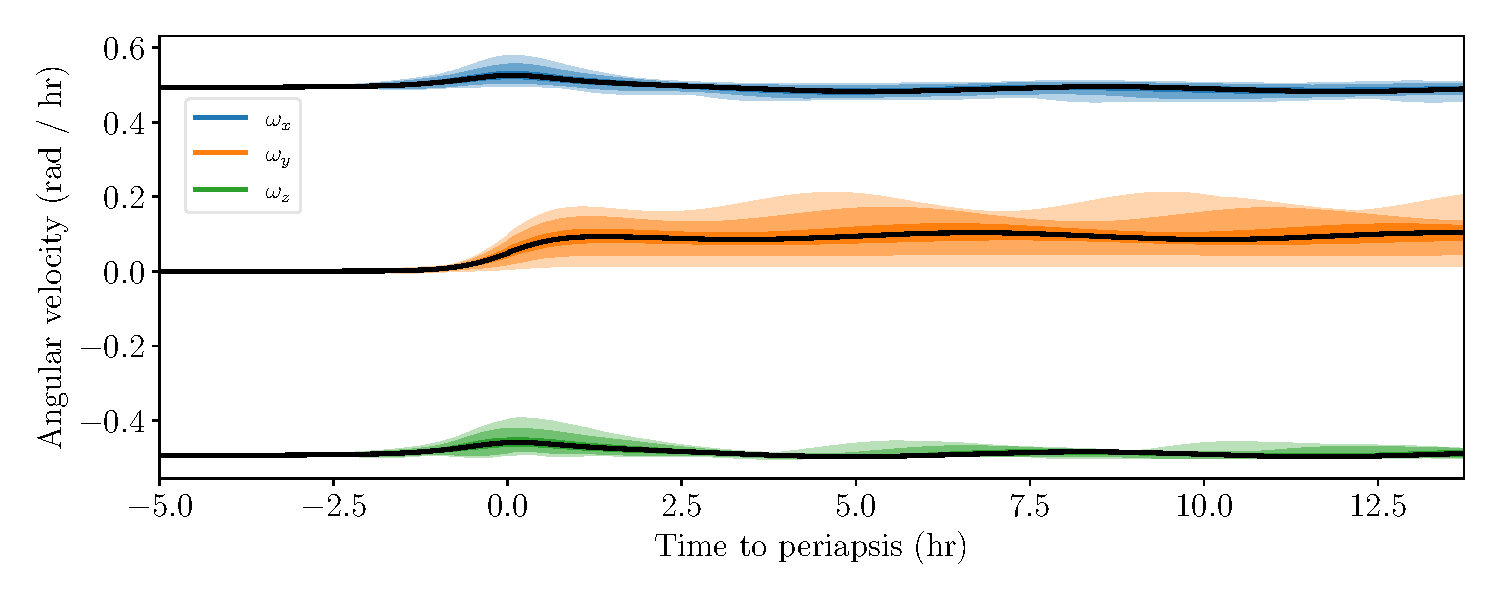
\includegraphics[width=0.7\textwidth]{nominal-data-sym.pdf}
  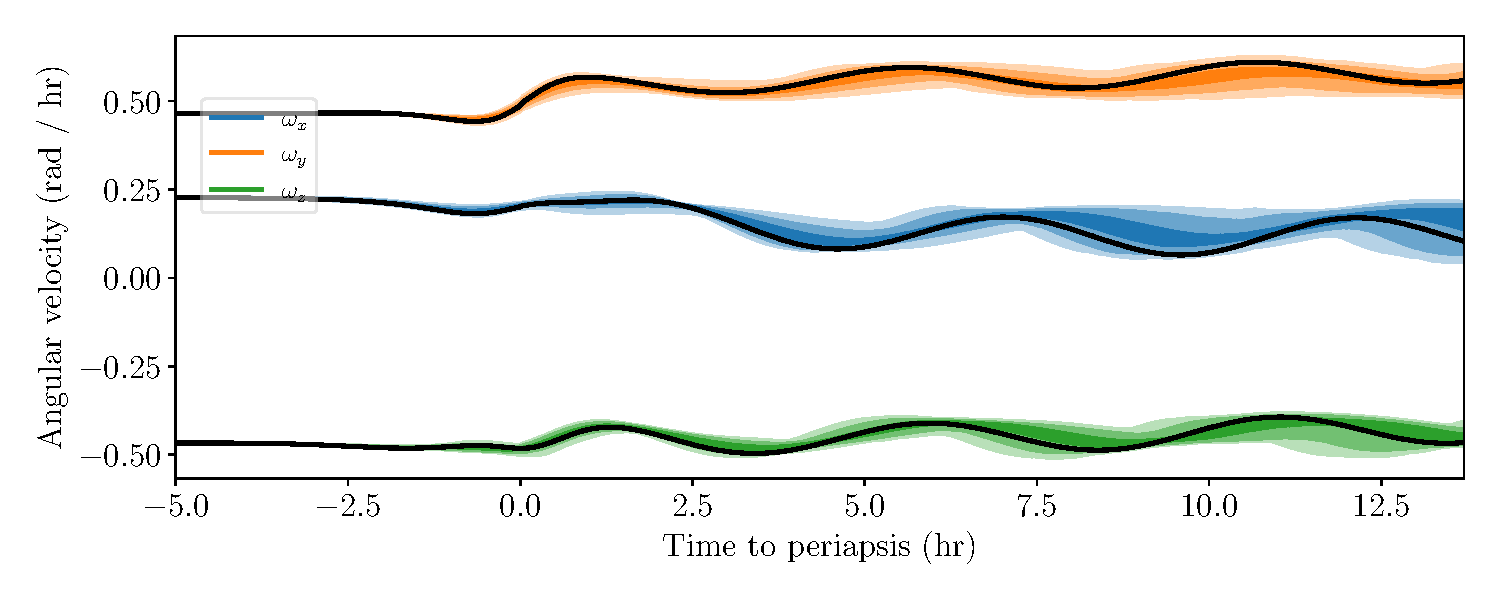
\includegraphics[width=0.7\textwidth]{nominal-data-asym.pdf}
  \caption{Angular velocity data simulated for the symmetric (above) and asymmetric (below) reference asteroid densities and the reference orbit (black lines). Also plotted is the deviation of the data for likelihood-distributed changes to the asteroid shape (bands) using the nominal uncertainty method. Bands contain 68.3\%, 95.5\%, and 99.7\% of the 1000 simulations run.}
  \label{fig:example-data}
\end{figure}


\subsubsection{Position dependent method}
In practice, precision on the asteroid spin axis will increase with decreasing distance \jtd{Citation needed}. The nominal sensitivity model does not account for this; however, we can approximate this effect by choosing $\sigma_\theta$ from the nominal method to be position-dependent. Specifically, we choose
\begin{equation}
\sigma_\theta(D) = unimplemented.
\label{eqn:pos-dependent-sensitivity}
\end{equation}
We do not expect this change to differ qualitatively from the nominal method because resolution is most important near pericenter, where $D$ is stationary to first order.



\subsection{System Setup}
We study several environments for our asteroid, including (1) a flyby of a single, spherical planet, (2) a close flyby of a ringed planet, (3) a flyby of a planet with a moon, and (4) a close flyby of a planet with a moon. The qualitative and quantitative differences between these flyby types are discussed below.

\subsubsection{One Spherical Planet}
The simplest setup for an asteroid flyby is a close flyby of a single, spherical body. We call this central body a ``planet'' because it is likely that a body massive enough to observably torque an asteroid would be a planet. For such a body, the only relevant physical parameter is its mass, $\mu_M$, since $J_{00} = 1$ and the other $J_{\ell m}$ parameters are zero.

\subsubsection{Ringed Planet}
Equation \ref{eqn:tidal-torque} demonstrates that parameters controlling non-sphericity in the central body ($J_{2m}$, $J_{3m}$, etc.) are damped by a factor of $(a_M/D)^\ell$, where $a_M$ can be thought to be the radius of the central body. Furthermore, the $J_{1m}$ terms are all zero by choosing the center of mass of the central body to be the origin of the coordinate system. Thus, we are interested in the extreme values of $J_{\ell \geq 2}$ and whether they have a significant effect on the observability of asteroid density distributions. An example of such an extreme value is the presence of a planetary ring.

For a ring of inner radius $a$, outer radius $b$, and mass $\mu_r$ oriented in the $\unit X-\unit Y$ plane, the only changed $J_{\ell m}$s have $m = 0$ by rotational symmetry. Furthermore, $Y_{\ell, m} = 0$ on the equator for odd $m$, and $(-1)^{\ell/2} \ell! / (2^\ell (\ell/2)!^2)$ otherwise. Thus, we have
\begin{equation}
J_{\ell m} = \left\{\begin{array}{cc}
\frac{2 \pi \sigma}{\mu_M + \pi(b^2-a^2)\sigma}\frac{(-1)^{\ell/2}}{a_M^\ell}\frac{b^{\ell+2} - a^{\ell+2}}{2^\ell (\ell/2)!^2 (\ell + 2)}
 & \text{for}\ m = 0,\ l\ \text{even},\ l \neq 0\\
1 & \ell = 1\\
0 & \text{else}
\end{array}\right.
\label{eqn:ring-jlm}
\end{equation}
where $\mu_M$ is the mass of the planet without the ring and $\sigma_s$ is the surface density of the ring.


The oblateness $\epsilon$, also called $J_2$ of a body is defined as $\epsilon = (I_z - I_x)/(\mu_M a_M^2)$, where $I_x = I_y$ (that is, $J_{22} = 0$) and $a_M$ is the true radius of the body, not the value defined in equation \ref{eqn:am}. Expressed in terms of $J_{\ell m}$, this is $\epsilon = -2J_{20}$. We can compare typical oblateness to the $J_{20}$ value from equation \ref{eqn:ring-jlm} to see which effect is more dramatic.

Using data from the NASA Saturn Fact Sheet, we arrive at $J_{20}\sim 10^{-8}$ from rings, but $10^{-4}$ from oblateness. So oblateness is in fact the stronger effect.

\jtd{Don't actually use this section in the paper. I'm keeping it here as a math repository. Change the section to an oblate planet.}

\subsection{Planet with a Moon: Distant Flyby}
Consider a system with a moon of mass $\mu_{o}$ at constant displacement $\bm R$ from the central body. We assume that both the planet and the moon are spherical. As long as the distance from the barycenter of the planet-moon system to the asteroid $D$ always satisfies $D>r$ we are free to use the formalism developed above, absorbing the moon into $J_{\ell m}$. Making use of the identity \cite{Gelderen1998TheSO}
\begin{equation}
R_{\ell m}(\bm R + \bm R') = \sum_{\ell' = 0}^\ell \sum_{m'=-\ell'}^\ell R_{\ell' m'}(\bm R') R_{\ell-\ell', m-m'}(\bm R)
\end{equation}
\jtd{Is this true?}
for $R > R'$, we have
\begin{equation}
J_{\ell m} = \frac{1}{(\mu_M+\mu_0) a_M^\ell}\brackets{\delta_{\ell 0}\delta_{m0}\mu_M + \int_\mathcal{P} d^3 r' \rho_o(\bm r') R_{\ell m}(\bm R + \bm r')}
\end{equation}
\begin{equation}
J_{\ell m} = \frac{1}{(\mu_M+\mu_0)}\brackets{\mu_M\delta_{\ell 0}\delta_{m0} + \mu_o \frac{R_{\ell m}(\bm R)}{ a_M^\ell}}
\end{equation}
where the $\delta$s are Kronecker deltas. It is apparent that if $a_M^\ell$ remains the radius of the planet, $|J_{\ell m}| \rightarrow \infty$ as $\ell \rightarrow \infty$. However, since each $J_{\ell m}$ is damped by $a_M^\ell / D^\ell$ and since $R < D$ by construction, the series in equation \ref{eqn:tidal-torque} remains roughly geometric and does not blow up. For the sake of this calculation, we neglect motion of the moon during the flyby.

For our tests, we use parameters similar to our Moon: we set $\mu_o = 0.01 \mu_M$ and $R = 60 a_M$.


\subsection{Planet with a Moon: Close Flyby}
If, contrary to the previous section, we want to fly by both the moon and the planet of a binary system, we must consider the tidal torque contributions from both bodies separately. The formalism above cannot be extended to write one set of $J_{\ell m}$ for both the moon and planet. To do this, we generate two separate paths of $\bm D(t)$, one pointing from the central body to the asteroid and one pointing from the moon the asteroid. Both are defined in the inertial reference frames. Then the torque from both can be computed by equation \ref{eqn:tidal-torque} and added to get the net torque on the asteroid. Again, we neglect motion of the moon during the flyby.



\section{Results}
To interpret the capacity of this tidal torque technique to constrain the density distribution of asteroids, we generate synthetic data in multiple simulated settings and fit to this data using an MCMC, reporting the standard deviation of the posterior parameter distributions as a measure of the effectiveness of the fit. Fits with narrow posterior distributions are considered more effective than those with wide posterior distributions, and the correlations between parameters are also of interest when computing uncertainties on physical models for the asteroid shape.

The distributions are nearly Gaussian in most cases (see appendix \ref{app:gaussian-posteriors}) and all fits are run until convergence.

\subsection{Dependence on asteroid parameters}
\label{sec:probe-space}
Of first importance is the dependence of parameter uncertainties on the true parameter values. To measure this, we run 120 fits, all for the two $K_{\ell = 2}$ parameters and $\gamma_0$ with the standard orbit (appendix \ref{app:standard}) and experimental uncertainty $\sigma_\theta = 0.01$ with the nominal uncertainty model(section \ref{sec:uncertainty-models}). Each fit is run for $\gamma_0=\pi/8$ and $K_{20}, K_{22}$ distributed in a triangular lattice with 17 layers, spanning the parameter space. The 33 cases with extremal values of $K_{22}$ are not fitted as being too close to the edge of the parameter space.

The parameters $K_{22}$ and $K_{20}$ are then converted to the more physical parameters $a/c$ and $b/c$ under the assumption of an elliptical asteroid of uniform density with minor axes $a, b, c$ (section \ref{sec:constant-density-ellipsoid}). Uncertainties on $\gamma_0$ and the two shape parameters are given in figure \ref{fig:probe-space-sigma}, and correlations between pairs of parameters ($\mathrm{Corr}(X, Y) = \mathrm{Var}(X, Y) / (\sigma_X \sigma_Y)$ are given in figure \ref{fig:probe-space-corr}. 
\begin{figure}
  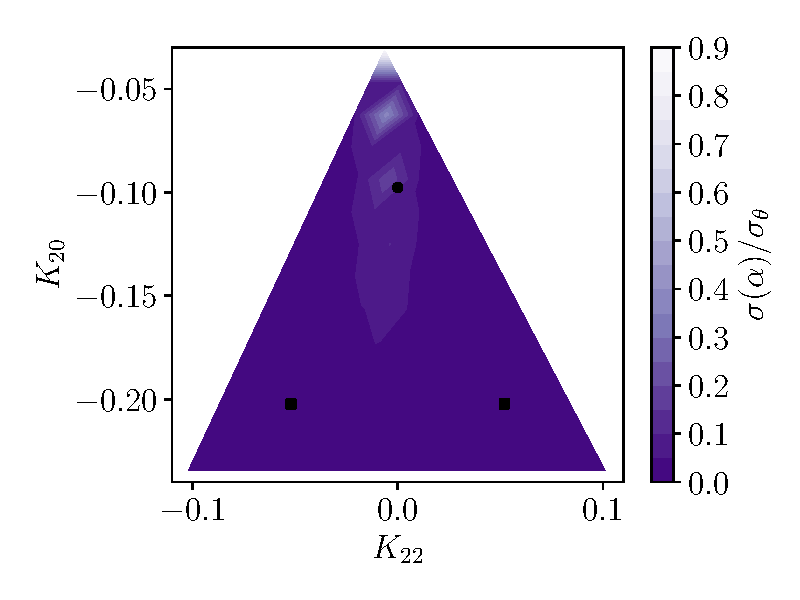
\includegraphics[width=0.33\textwidth]{probe-space-theta-1-sigma.pdf}\hfill
  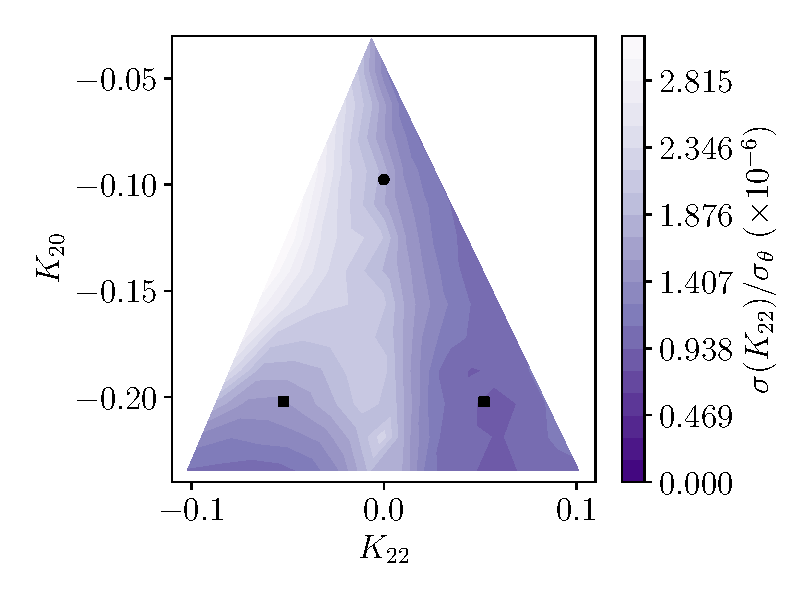
\includegraphics[width=0.33\textwidth]{probe-space-theta-2-sigma.pdf}\hfill
  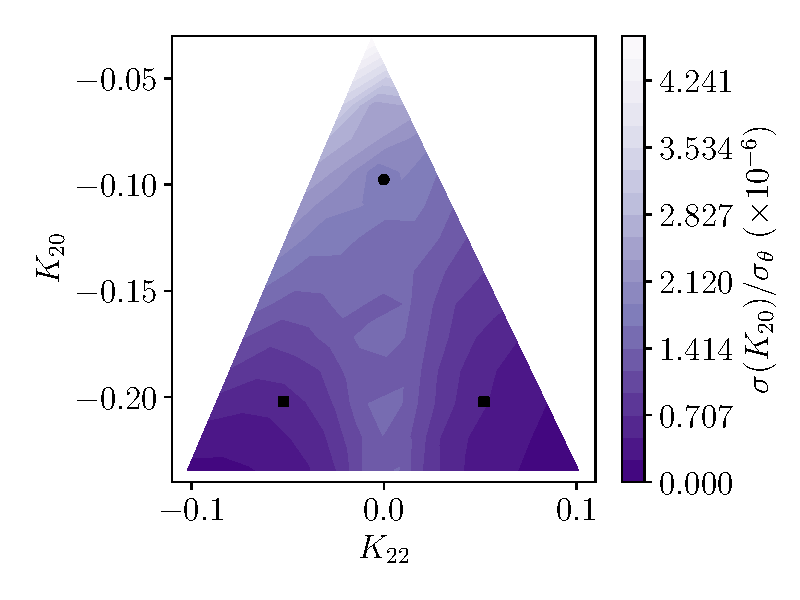
\includegraphics[width=0.33\textwidth]{probe-space-theta-3-sigma.pdf}

  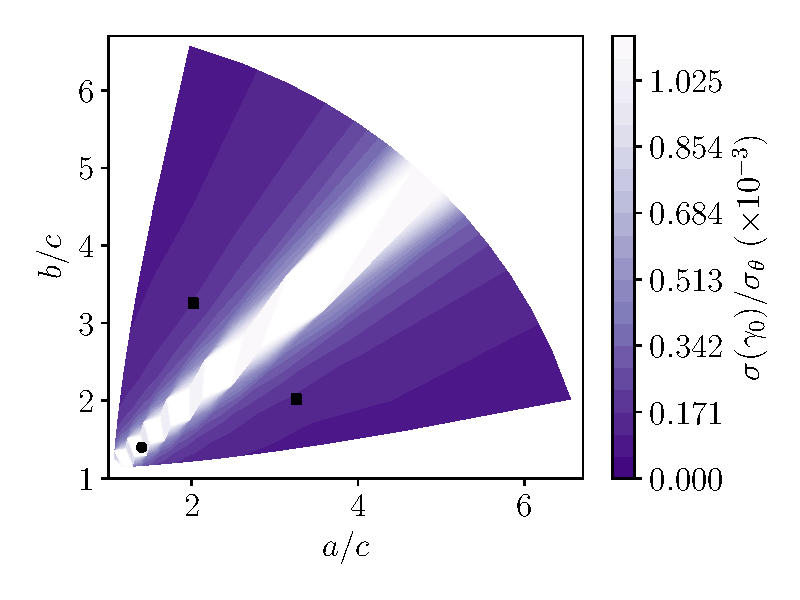
\includegraphics[width=0.33\textwidth]{probe-space-ab-1-sigma.pdf}\hfill
  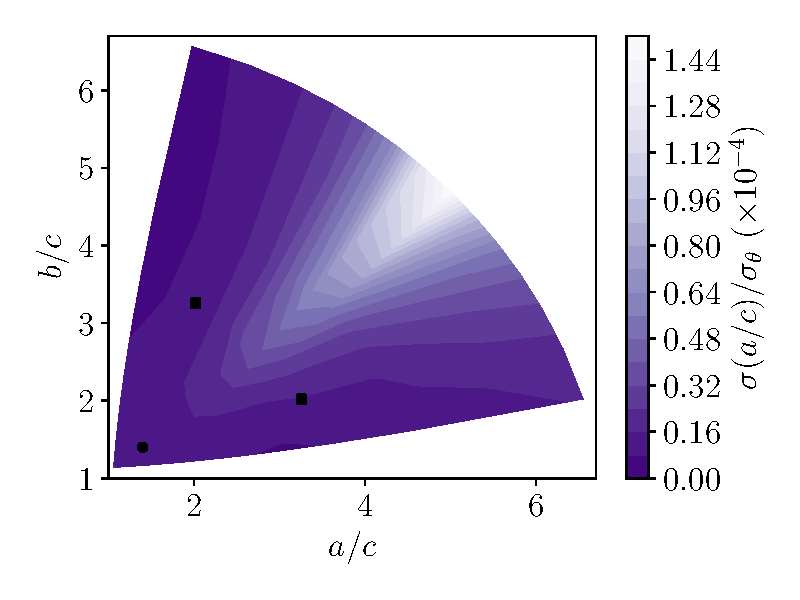
\includegraphics[width=0.33\textwidth]{probe-space-ab-a-sigma.pdf}\hfill
  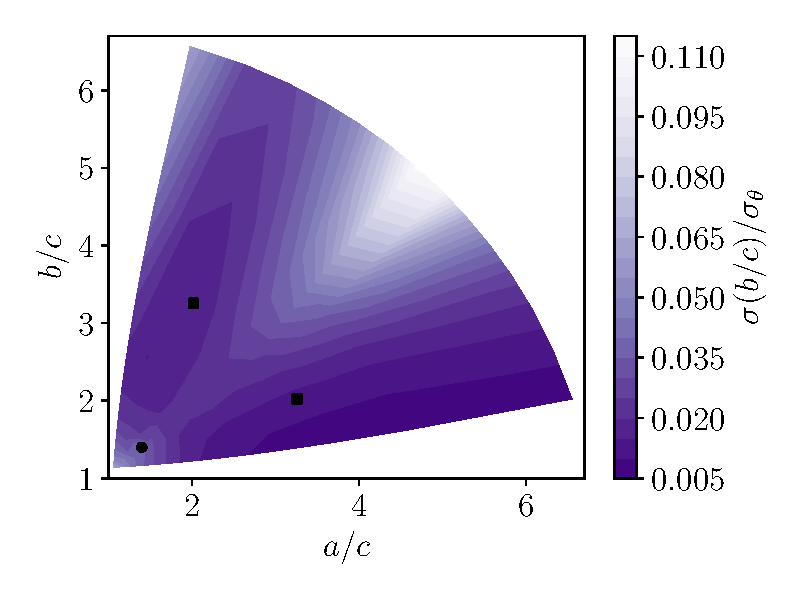
\includegraphics[width=0.33\textwidth]{probe-space-ab-b-sigma.pdf}

  \caption{Ratios of fit uncertainties (the standard deviations of parameter posterior distributions) to experimental uncertainty ($\sigma_\theta$) for fit parameters $\gamma_0$, $K_{22}$, and $K_{20}$ (top row) and $\gamma_0$, $a/c$, and $b/c$ (bottom row). Also shown are the reference asteroid shapes used elsewhere in this paper (appendix \ref{app:reference-config}); the symmetric case is marked with a circle and the asymmetric with a square.}
  \label{fig:probe-space-sigma}
\end{figure}

\begin{figure}
  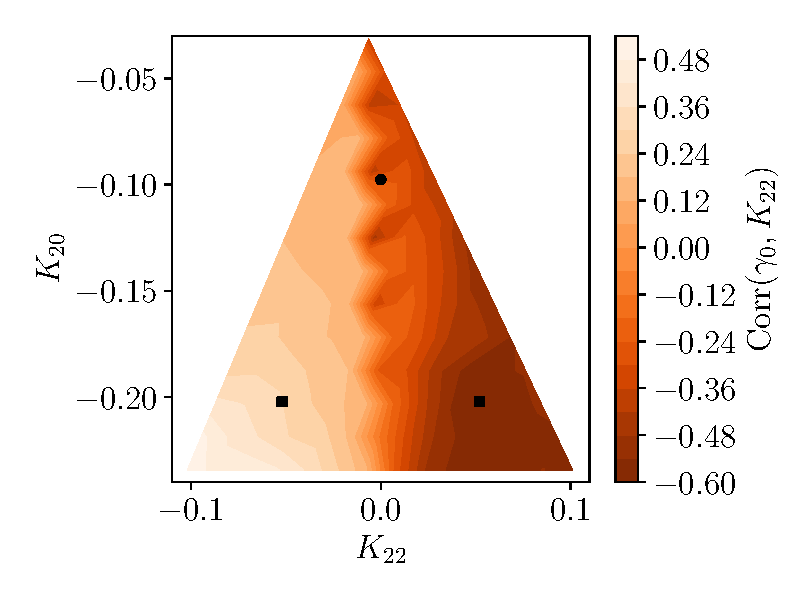
\includegraphics[width=0.33\textwidth]{probe-space-corr12.pdf}\hfill
  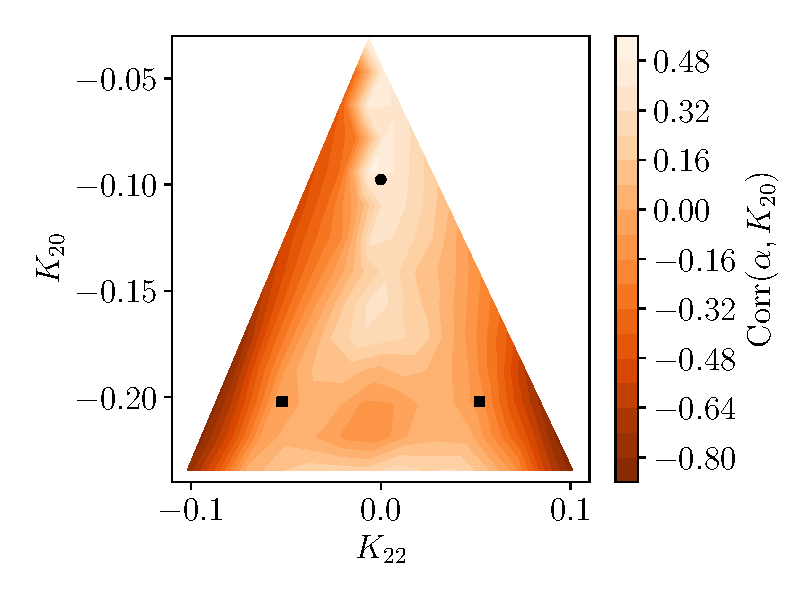
\includegraphics[width=0.33\textwidth]{probe-space-corr13.pdf}\hfill
  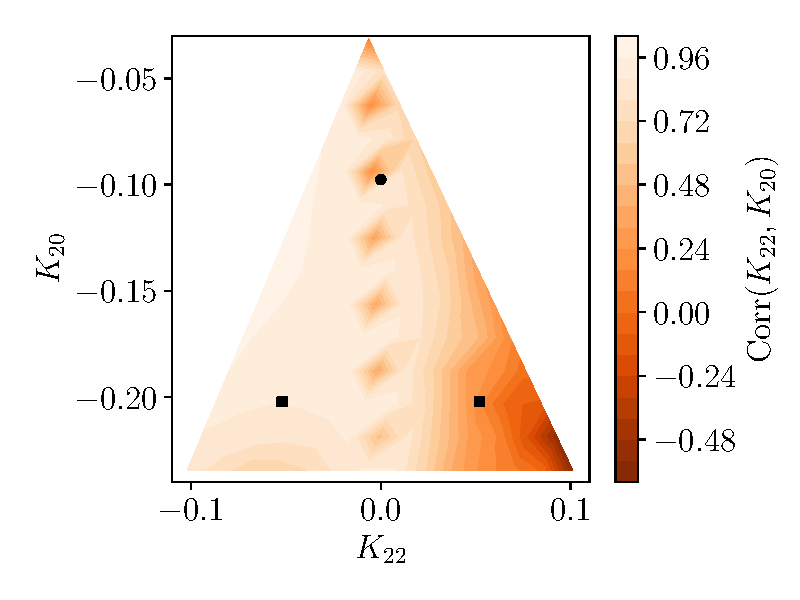
\includegraphics[width=0.33\textwidth]{probe-space-corr23.pdf}
  
  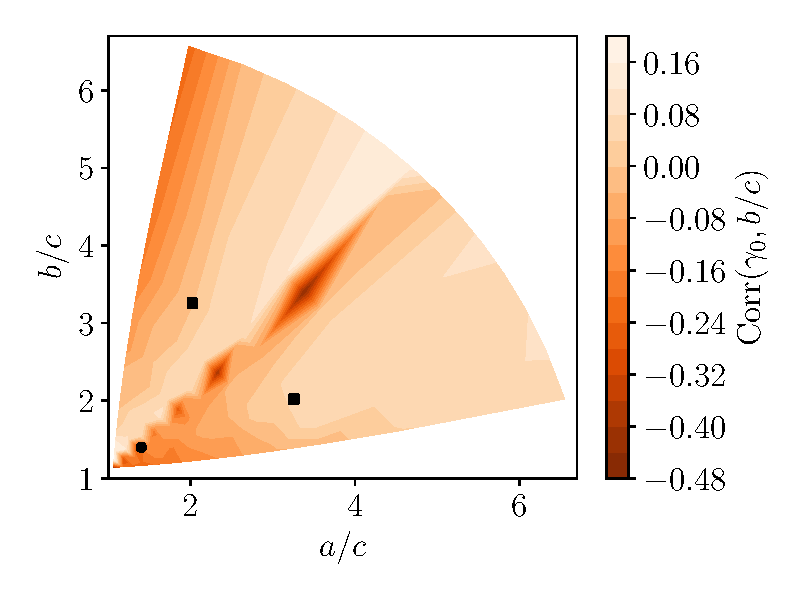
\includegraphics[width=0.33\textwidth]{probe-space-ab-1b.pdf}\hfill
  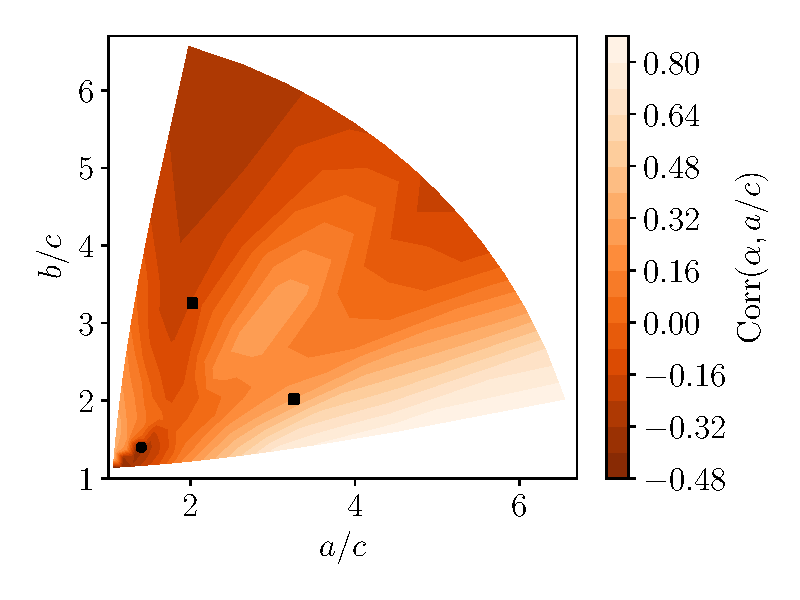
\includegraphics[width=0.33\textwidth]{probe-space-ab-1a.pdf}\hfill
  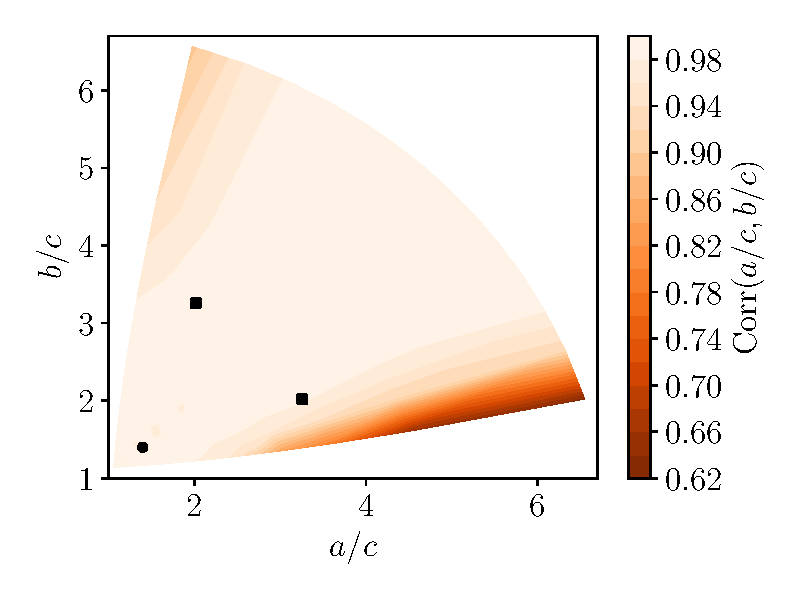
\includegraphics[width=0.33\textwidth]{probe-space-ab-ab.pdf}
  
  \caption{Correlations between fit uncertainties and experimental uncertainty ($\sigma_\theta$) for fit parameters $\gamma_0$, $K_{22}$, and $K_{20}$ (top row) and $\gamma_0$, $a/c$, and $b/c$ (bottom row). Also shown are the reference asteroid shapes used elsewhere in this paper (appendix \ref{app:reference-config}); the symmetric case is marked with a circle and the asymmetric with a square.}
  \label{fig:probe-space-corr}
\end{figure}

These figures demonstrate several key properties. Figure \ref{fig:probe-space-sigma} demonstrates that fit uncertainties for all three parameters are generally for asteroids with an axis of rotational symmetry --- i.e. $a=b$ or $K_{22} = 0$. This is likely due to the fact that the local axes, which are required to define the parameters, are set such that they align with the asteroid principal axes, and therefore are degenerate in the case of a symmetrical asteroid. For similar reasons, uncertainty in $\gamma_0$ especially is large for $a \approx b \approx c$, which is the spherical case in which no tidal torque is generated. Beyond these two trends, uncertainty in $a/c$ and $b/c$ appear to scale linearly with these ratios. 

Figure \ref{fig:probe-space-corr} demonstrates that the parameters are generally correlated. Specifically, $\gamma_0$ and $|K_{22}|$ are correlated for large $|K_{22}|$ which corresponds to highly asymmetric asteroids. Likewise, for the correlation of $a/c$ and $b/c$ with $\gamma_0$. $\mathrm{Corr}(\gamma_0, K_{20})$ is less, however. $K_{20}$ and $K_{22}$ are strongly correlated in general as are $a/c$ and $b/c$.

Also shown in figures \ref{fig:probe-space-sigma} and \ref{fig:probe-space-corr} are the reference asteroid configurations which we study when fixing the asteroid shape and varying other parameters. We note that these reference configurations capture the above trends in variance and correlation, so that they can be viewed as representative of all but the most extreme asteroid configurations. The measured values of variance and covariance are displayed in table \ref{tab:probe-space-refernece-var-covar}.

\begin{table}
  \centering
  \begin{tabular}{c c c c c c c}
    \hline \hline
    Benchmark configurations & $\sigma(\gamma_0)$ / $\sigma_\theta$ & $\sigma(K_{22}\ [a/c])$ / $\sigma_\theta$ & $\sigma(K_{20}\ [b/c])$ / $\sigma_\theta$ & $\mathrm{Corr(\gamma_0, K_{22})}$ & $\mathrm{Corr(\gamma_0, K_{20})}$ & $\mathrm{Corr(K_{22}, K_{20})}$ \\ \hline
    Symmetric: $a=b$ & 36 & $1.9 \times 10^{-6}$ & $1.7 \times 10^{-5}$ & -0.40 & 0.36 & 0.19\\%24
    & 36 & $9.4\times 10^{-5}$ & $1.9\times 10^{-4}$ & -0.42 & -0.29 & 0.96 \\
    Asymmetric: $a<b$ & $1.6 \times 10^{-5}$ & $1.5 \times 10^{-6}$ & $5.4 \times 10^{-6}$ & 0.32 & -0.0053 & 0.88\\%94
    & $1.6\times 10^{-5}$ & $9.4\times 10^{-5}$ & $1.8\times 10^{-4}$ & 0.082 & -0.019 & 0.99\\
    Asymmetric: $a>b$  & $1.5 \times 10^{-5}$ & $9.1 \times 10^{-7}$ & $4.8 \times 10^{-6}$ & -0.58 & 0.017 & 0.15 \\%101
    & $1.5\times 10^{-5}$ & $1.5\times 10^{-4}$ & $1.0\times 10^{-4}$ & -0.049 & 0.061 & 0.98\\ \hline
  \end{tabular}
  \caption{Values for the standard deviation and correlation of $\gamma_0$, $K_{22}$, and $K_{20}$ (top entry of each row) or $\gamma_0$, $a/c$, and $b/c$ respectively (bottom entry of each row) for the symmetric and asymmetric reference points. The large $\sigma(\gamma_0)$ for the symmetric benchmark reflects the fact that $\gamma_0$ is not defined for a symmetric body, and the posterior probability distribution is poorly constrained.}
  \label{tab:probe-space-refernece-var-covar}
\end{table}


\subsection{Dependence on observational precision}
\label{sec:probe-sigma}

Depending on the size of the asteroid, its orbital elements, and the availability of observation, uncertainty on the rotational pole of the asteroid is expected to vary between flybys. A detailed model of uncertainty in the rotational pole of the asteroid (a model that might simulate a full lightcurve, for example) is beyond the scope of this paper. However, in this section we demonstrate how the uncertainty in the fit parameters is governed by the experimental uncertainty in rotational pole $\sigma_\theta$ as a rule-of-thumb to guide future investigation.

We represent 1-$\sigma$ uncertainty in the fit parameters as the difference between the 84th or 15th percentile of the marginal posterior PDF for each fit parameter and its mean. For a multivariate gaussian posterior PDF (which must also have gaussian marginal PDFs), this 1-$\sigma$ uncertainty is exactly the standard deviation of the marginal PDF. We perform a similar exercise for the 2-$\sigma$ uncertainty.

These uncertainties in fit parameters are observed to scale precisely with $\sigma_\theta$, except where $\sigma_\theta$ is large enough that the fit parameter uncertainty is comparable to the size of the prior PDF. Figure \ref{fig:probe-sigma} shows the $\sigma / \sigma_\theta$ ratio for all 10 of the first two orders of parameters ($\gamma_0$, $K_{2m}$, and $K_{3m}$). The ratio of $\sigma_\rho$ to $\sigma_\theta$ is kept constant. The result is executed for the asymmetric asteroid model. The figure demonstrates that the ratio $\sigma/\sigma_\theta$ is constant for all values of $\sigma_\theta$ except large values. It also demonstrates that the posterior marginal PDFs are largely symmetric, in that the lower uncertainty is roughly equal to the upper uncertainty.

\begin{figure}
  \centering
  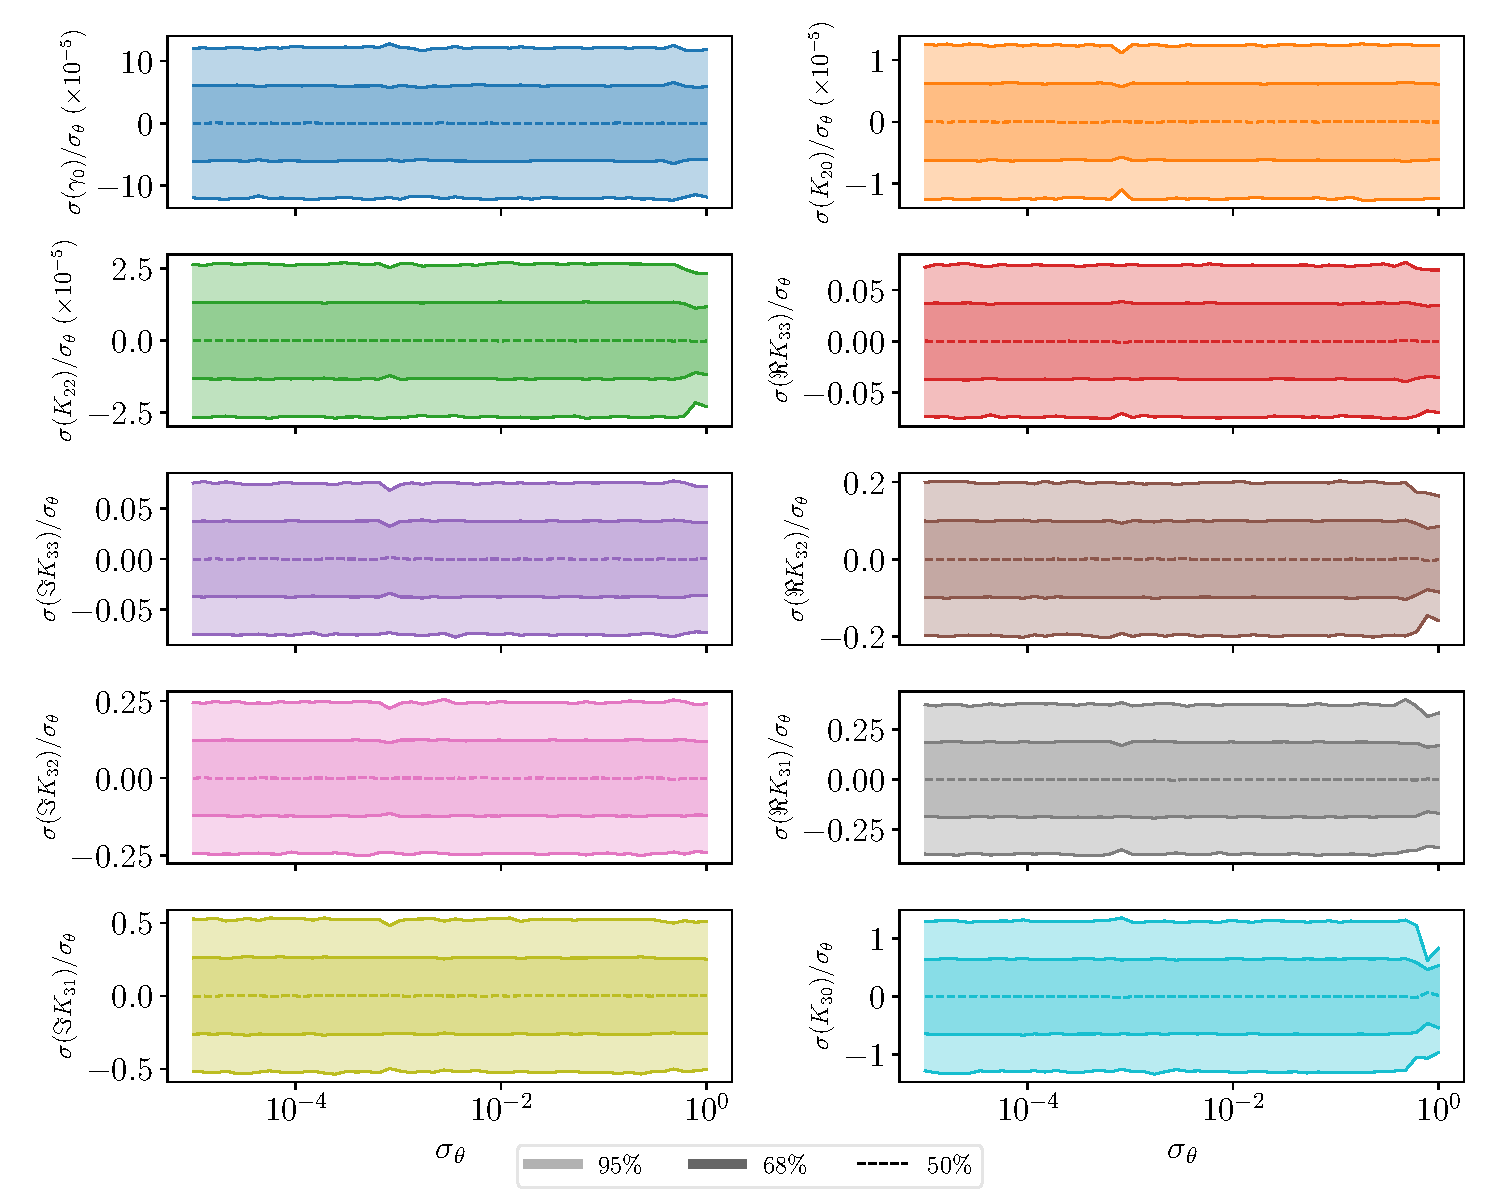
\includegraphics[width=0.8\textwidth]{probe-sigma.pdf}
  \caption{Ratio of 1- and 2-$\sigma$ uncertainties of the marginal PDFs to the observational uncertainty $\sigma_\theta$ as a function of $\sigma_\theta$. Except at large $\sigma_\theta$, the ratio is observed to be constant. The asymmetric asteroid benchmark is used. Values of the ratio for other asteroid models can be computed from figure \ref{fig:probe-space-sigma}.}
  \label{fig:probe-sigma}
\end{figure}

Due to the constancy of the ratio of fit to observational uncertainty, the ratio can be extracted for other asteroid configurations from figure \ref{fig:probe-space-sigma}, and we are not much concerned with the value of $\sigma_\theta$ used throughout this paper because we are aware that results can be easily rescaled.


\subsection{Dependence on cadence}


\subsection{Dependence on orbital parameters}

\jtd{Do v and rp separately? Perhaps do not map}

\subsection{Dependence on spin pole}

\jtd{The period is also important, but probably depends too much on the start of the simulation. I'm more interested in the spin pole.}


\subsection{Dependence on blocking out perigee}
\label{sec:block-perigee}
Much of the data available concerning an asteroid's rotational velocity is captured much before or much after the flyby perigee, where tidal torque is low. The angular velocity evolution here is dominated by torque-free precession dictated by the moment of inertia components, so that zero-torque data can still be used to fix $K_{20}$ and $K_{22}$. However, $K_{3m}$ are not extractable from precession data alone. We are therefore curious how much of the sensitivity of the system to $K_{3m}$ components is due only data taken during the encounter perigee.

To test this, we mask the perigee of the counter by removing data from the period when $D < f_\textrm{mask} r_p$, where $f_\textrm{mask}>1$ is a unit-less fraction. We also allow the simulation to continue beyond the standard $f = 10$, so that the actual length of the data set is unaffected by the mask and induces no lack of precision on the fit of $K_{3m}$. We then fit to synthetic data for each mask and plot the standard deviations of the parameter posterior PDFs for (1) $\gamma_0$ and $K_{2m}$ as a control, and (2) $K_{3m}$, to test whether they can still be fitted for without data concerning the perigee. To maximize the changes in posterior PDF, we use an experimental error of $\sigma_\theta = 10^{-5}$, the lowest we test in this study.

\subsection{Exotic scenarios}

\subsubsection{Oblate planet}

\subsubsection{Distant moon}

\subsubsection{Close moon}




\section{Interpretation of the Fit Parameters}
The physical parameters $K_{\ell m}$ resulting from a fit to flyby data, while physical, do not completely describe an asteroid. Since the density distribution of the asteroid has many more degrees of freedom in general than the number of known $K_{\ell m}$, there are often many degenerate density distributions associated with one set of $K_{\ell m}$. As an example, consider a spherical asteroid of radius $A$ and density distribution of the form $\rho(\bm r) = \sum_{\ell m} f_{\ell m}(r) Y_{\ell m}^*(\unit r)$. Then we have
\begin{equation}
K_{\ell m} = N_{\ell m} \frac{(-1)^m}{(\ell + m)!(\mu_m a_m^\ell)}\int_0^A r^{2+\ell} dr f_{\ell m}(r)
\end{equation}
where $N_{\ell m}$ is given by equation \ref{eqn:nlm}. Thus, $K_{\ell m}$ constrains only the integrals of $f_{\ell m}$, not the functions themselves. By relaxing the assumption that the asteroid is a sphere, even more degeneracy is introduced.

To avoid this degeneracy, we either (1) assume that the density is constant and solve for the asteroid surface (section \ref{sec:constant-density}), (2) assume that the surface of the asteroid is fixed and solve for $\rho(\bm r)$. In the latter case, we can avoid the above degeneracy either by assuming $\nabla^2 \rho = 0$ (section \ref{sec:laplace-rho}) or by using a numerical approach to find a more characteristic density distribution (section \ref{sec:numerical-density}).

\jtd{Not all of these models will be in the paper. This is a list of all the models I've thought of. I'll give some examples of applying these models to ``realistic'' asteroid density profiles (uniform, regolith over rock, etc) and see what they get, using that filter to describe the best.}

\subsection{Constant Density Asteroid Model}
\label{sec:constant-density}
Suppose our asteroid has constant density $\rho_0$ and known parameters $K_{\ell m}$ and $a_m$. We do not expect to solve for $\rho_0$ or equivalently $\mu_m$ since the mass of the asteroid cannot be extracted from tidal torque. However, we can solve for the asteroid shape required to match the known $K_{\ell m}$. In this process, we ignore $a_m$ until the last step, when we rescale the asteroid shape model until the correct $a_m$ is yielded.

Suppose the asteroid is ``star shaped'' in that every point on its surface maps to a unique set of spherical coordinates $\theta, \phi$, and $r(\theta, \phi)$. We use the helpful identity
\begin{equation}
  K_{\ell m} = \frac{\rho_m}{\mu_m a_m^\ell} \int_\mathcal{A} d^3 r R_{\ell m} (\bm r)
   = \frac{\rho_m}{\mu_m a_m^\ell} \int_\mathcal{A} d^3 r \nabla \cdot \bm v (\bm r)
    = \frac{\rho_m}{\mu_m a_m^\ell} \oint_{\partial \mathcal{A}} d^2 \bm r \cdot \bm v (\bm r)
\end{equation}
where $\bm v (\bm r) = \unit r R_{\ell m} (\bm r) r / (3+\ell) $. We know the area element satisfies $d^2 \bm r = \partial \bm r / \partial \theta \times \partial \bm r / \partial \phi$ in our coordinates, and when dotted with $\bm v \propto \unit r$, this gives
\begin{equation}
  K_{\ell m} = \frac{\rho_m}{\mu_m a_m^\ell(3 + \ell)} \int_0^\pi d\theta \sin \theta\int_0^{2\pi}d\phi r(\theta, \phi)^3 R_{\ell m}(r(\theta, \phi), \theta, \phi).
  \label{eqn:constant-density-klm}
\end{equation}
The integrand of each $K_{\ell m}$ therefore is proportional to $r(\theta, \phi)^(3+\ell)$ times constants and a spherical harmonic. We can write $r(\theta \phi) = \sum_{\ell m} Y_{\ell m}^* C_{\ell m}$ without loss of generality, in which case equation \ref{eqn:constant-density-klm} becomes a polynomial of degree $3+\ell$ in terms of $C_{\ell' m'}$ and integrals of products of spherical harmonics. These integrals can be precomputed, since they are taken over the whole sphere $\theta \in (0, \pi)$ and $\phi \in (0, 2\pi)$. Equation \ref{eqn:constant-density-klm} can then be numerically solved to get $C_{\ell m}$. Specifically, the ratios of $K_{\ell m} / K_{\ell 0}$ can be solved for to eliminate the prefactor, then $\rho_m / \mu_m$ chosen such that $K_{00} = 1$. If $n$ values of $K_{\ell m}$ are known, then this method solves exactly for $n$ values of $C_{\ell m}$.
\jtd{Implement this as a check.}


\subsubsection{Special Case: Constant Density Ellipsoid}
\label{sec:constant-density-ellipsoid}
Suppose that only $K_{\ell = 2}$ are known. Then the above method is not necessary to compute the uniform density shape; we can assume the asteroid is an ellipsoid and solve for the axis lengths, which are
\begin{equation}
a = \sqrt{\frac{5}{3}}a_m\sqrt{1-2K_{20}+12K_{22}} \qquad b = \sqrt{\frac{5}{3}}a_m\sqrt{1-2K_{20}-12K_{22}} \qquad c = \sqrt{\frac{5}{3}}a_m\sqrt{1+4K_{20}}.
\label{eqn:ellipsoid-klm}
\end{equation}
These arise out of computing the moments of inertia for a constant density ellipsoid and using equation \ref{eqn:moi} to relate the result to $K_{\ell m}$ and $a_m$. The values $a$, $b$, and $c$, represent semi-axes aligned with $\unit x$, $\unit y$, and $\unit z$ respectively.

Again, the density of this asteroid cannot be extracted because, as is a general principle of gravitational interactions, the mass of the asteroid does not affect its dynamics. If $a_m$ is unknown, the ratios $a/c$ and $b/c$ can be computed instead. Since $I_{zz}$, is the greatest of the moments of inertia, we expect $a/c > 1$ and $b/c > 1$. 


\subsection{Fixed Surface $\nabla^2 \rho = 0$ model}
\label{sec:laplace-rho}
Now suppose the shape of the asteroid is known, perhaps by a simplifying guess or perhaps by direct observation during a flyby. Then a density distribution $\rho(\bm r)$ can be solved for which is consistent with observed values of $K_{\ell m}$. Supposing $\nabla^2 \rho = 0$ and removing terms which are undefined at $r=0$, we write $\rho(\bm r) = \sum_{\ell m} C_{\ell m} R_{\ell m}^* a_m^\ell \mu_m$. Thus, $K_{\ell m} = \sum_{\ell' m'} C_{\ell' m'} B_{\ell \ell' m m'}$ where
\begin{equation}
  B_{\ell \ell' m m'} = \int_{\mathcal{A}}d^3 r R_{\ell m}(\bm r) R_{\ell' m')}(\bm r)
  \label{eqn:blm}
\end{equation}
can be precomputeded due to the shape of $\mathcal{A}$ being known.
If we write $K_{\ell m}$ as a vector $\bm K$ and similarly for $\bm C$, we can write $B_{\ell \ell' m m'}$ as a matrix $\hat B$, obtaining $\bm K = \hat B \bm C$. It follows that the density distribution coefficients are given by
\begin{equation}
\bm C = \hat B^{-1} \bm K.
\end{equation}
The scale parameter $a_m$ can be computed from the resulting values of $\bm C$ and the distance scale can be adjusted until $a_m$ matches the true value. As before, $\mu_m$ is a free parameter representing the impossibility of fitting for the mass of the asteroid. Since only a finite number of $K_{\ell m}$ are known, we can only solve for a finite number of $C_{\ell m}$ and neglect the higher order terms.

Physically, there is no reason to expect $\nabla^2 \rho = 0$. However, the space of density distributions with $\nabla^2 \rho = 0$ is a useful proxy for the true density distribution, since this section demonstrates how the density distribution can be solved for within this subspace. Conceptually, the density distribution derived from the $C_{\ell m}$s can be viewed as a projection from the true density distribution into the closest density distribution with $\nabla^2 \rho = 0$ everywhere.

Note that if $\mathcal{A}$ is assumed to be a sphere, $B_{\ell \ell' m m'} \propto \delta_{\ell \ell'} \delta_{m m'}$ and $B_{\ell \ell m m}$ can be computed analytically. Thus, the matrix inversion step is not required in this case.

\subsection{Fixed Surface Numerical Model}
\label{sec:numerical-density}
Now we approach the problem of solving for the density distribution of an asteroid from the $K_{\ell m}$ parameters with more general assumptions. Suppose the shape of the asteroid is known, where ``known'' in this case means that an indicator function $\mathds{1}(\bm r)$ exists such that $\mathds{1}(\bm r) = 1$  inside the asteroid and 0 elsewhere. Then we suggest a numerical algorithm to compute a representative distribution of the asteroid density distribution. Given $n$ known values of $K_{\ell m}$, the algorithm proceeds as follows.
\begin{enumerate}
\item Fill the asteroids with $n$ uniformly random ``seed points'' by distributing them inside a bounding box containing the asteroid and rejecting those with positions $\bm r_i$ such that $\mathds{1}(\bm r_i) = 0.$
\item Construct $n$ regions $\mathcal{R}_i$around each point such that the $i$th region is the set of all points inside the asteroid closest to the $i$th point. Suppose $R_i$ has uniform density $\rho_i$.
\item For each region, compute $\overline K_{\ell m}^i = \frac{1}{\mu_m a_m^\ell}\int_{\mathcal{R}_i} d^3 r R_{\ell m}(\bm r)$. Once again, $\mu_m$ is a free parameter and units can be chosen such that $a_m=1$. Then %we can write $K_{\ell m} = \sum_i \rho_i \overline K_{\ell m}^i$.
\item Write $\overline K_{\ell m}^i$ as a square matrix $\hat{\overline K}$ with columns indexed by $i$ and rows indexed by $\ell$ and $m$. Invert it to get $\bm \rho = \hat {\overline K}^{-1} \bm K$.
\item Go back to step 1 and compute new density maps with new draws of seed points. Since $K_{\ell m}$ is linear in $\rho$, the average density distribution also satisfies the fitted $K_{\ell m}$. Use the average as the asteroid density distribution.
\end{enumerate}

\jtd{What does this give mathematically?}



\section{Uncertainty Testing}


\section{Conclusion}


\jtd{Talk about the walker spacing: the clamps, the scale with sigma, and the block diagonal hermitian matrices}

\jtd{Talk about first order torque}

\jtd{Talk about how numerical accuracy was chosen}

\jtd{Show plot of likelihood? (May not be necessary, since the corner plots are also shown)}

\jtd{Move up error bar section so that plots can be explained?}

\jtd{Compare the results to gaussians (they are not gaussian near the edges). Could do moment testing, or the Shapiro-Wilk test, which is frequentist so I don't want to do it.}

\jtd{Question: How to express non-gaussianity of distro?}
\jtd{Question: How important is it that the true value is not reproduced by the fit? Should I try to fix this? It's caused by the Gaussian approximation of the likelihood being incorrectm and by the fact that the data is not quite drawn from the distributions we model in the likeihood (it's drawn from the distribution of the true spin, not the data spin).}

\vspace{5mm}
\facilities{MIT Supercloud}

%% Similar to \facility{}, there is the optional \software command to allow 
%% authors a place to specify which programs were used during the creation of 
%% the manuscript. Authors should list each code and include either a
%% citation or url to the code inside ()s when available.

\software{emcee, scipy.optimize.minimize, numdifftools.Hessian}

\appendix

\section{Reference flyby configurations}
\label{app:reference-config}
Except when otherwise mentioned, we use the following fit parameters when running the simulation. Many of the parameter choices are made to maximize the quality of observations (a close orbit, large asteroid, etc.) This is so that if it is desired to test the dependence of fit results on perigee distance, for instance, the other parameters will not be fixed at values that are so unfavorable to observations that good fits are already excluded. Otherwise, the fit results for all perigee distances would always be poor and the dependence on perigee would be difficult to measure.
\begin{enumerate}
  \item An orbit around Earth with $6\siunit{km}\per{s}$ excess velocity and perigee at 5 Earth radii. \jtd{Cite Apophis close approach}
  \item An initial roll of $\gamma_0=\pi/8$.
  \item A cadence of 2 minutes and observational uncertainty of $\sigma_\theta = 0.01$ and $\sigma_\rho / \sigma_\theta = 10^{-5}$.
  \item A rotational period of 9 hours, with the rotational velocity vector distributed between the $\unit X$, $\unit Y$, and $\unit Z$ axes in a $1:2:-2$ ratio.
  \item An asteroid with radius $a_m = 1\siunit{km}$ and $K_{3m}=0$. For $K_{22}$ and $K_{20}$, we use two standard values. One with $(K_{22}, K_{20}) = (0, -0.097)$ and one with $(0.052, -0.202)$. Including the third point obtained by reflection $K_{22}\rightarrow -K_{22}$, these are the three points that minimize the mean distance between an arbitrary point in the allowed parameter space (equation \ref{eqn:parameter-bounds}) and these reference values. The first point is called the symmetric case because the corresponding uniform-density-ellipsoid model is rotationally symmetric around $\unit z$. The second case and its reflection are called the asymmetric cases. Values of $(0.052, -0.202)$ have $a < b$ in the ellipsoid model, and the reflected value has $a > b$. If not specified, we use the $a < b$ case. 
\end{enumerate}



\section{Example fit results}
In the interest of demonstrating the result of a fit to synthetic data, we present the results of a fit to synthetic data generated with the nominal sensitivity model and $\sigma_\theta = 10^{-5}$. The symmetric reference asteroid is used. The reduced $\chi^2$ value of this fit (defined as $\chi^2 / N$, where $N$ is the number of degrees of freedom) was 0.83, and fit results were in good agreement with the true parameters. Nearly 12,000 MCMC iterations were required before convergence.

Figure \ref{fig:example-residuals} shows the data with the best-fit overlaid and the residuals. Uncertainties are plotted on the residuals corresponding to the square root of the diagonal entries of the covariance matrix --- i.e., 1-$\sigma$ uncertainties. However, the data often exceeds these uncertainty bands. This is because uncertainties are correlated in truth, and points that fall outside of the band are not necessary in conflict with the best fit.

\begin{figure}
  \centering
  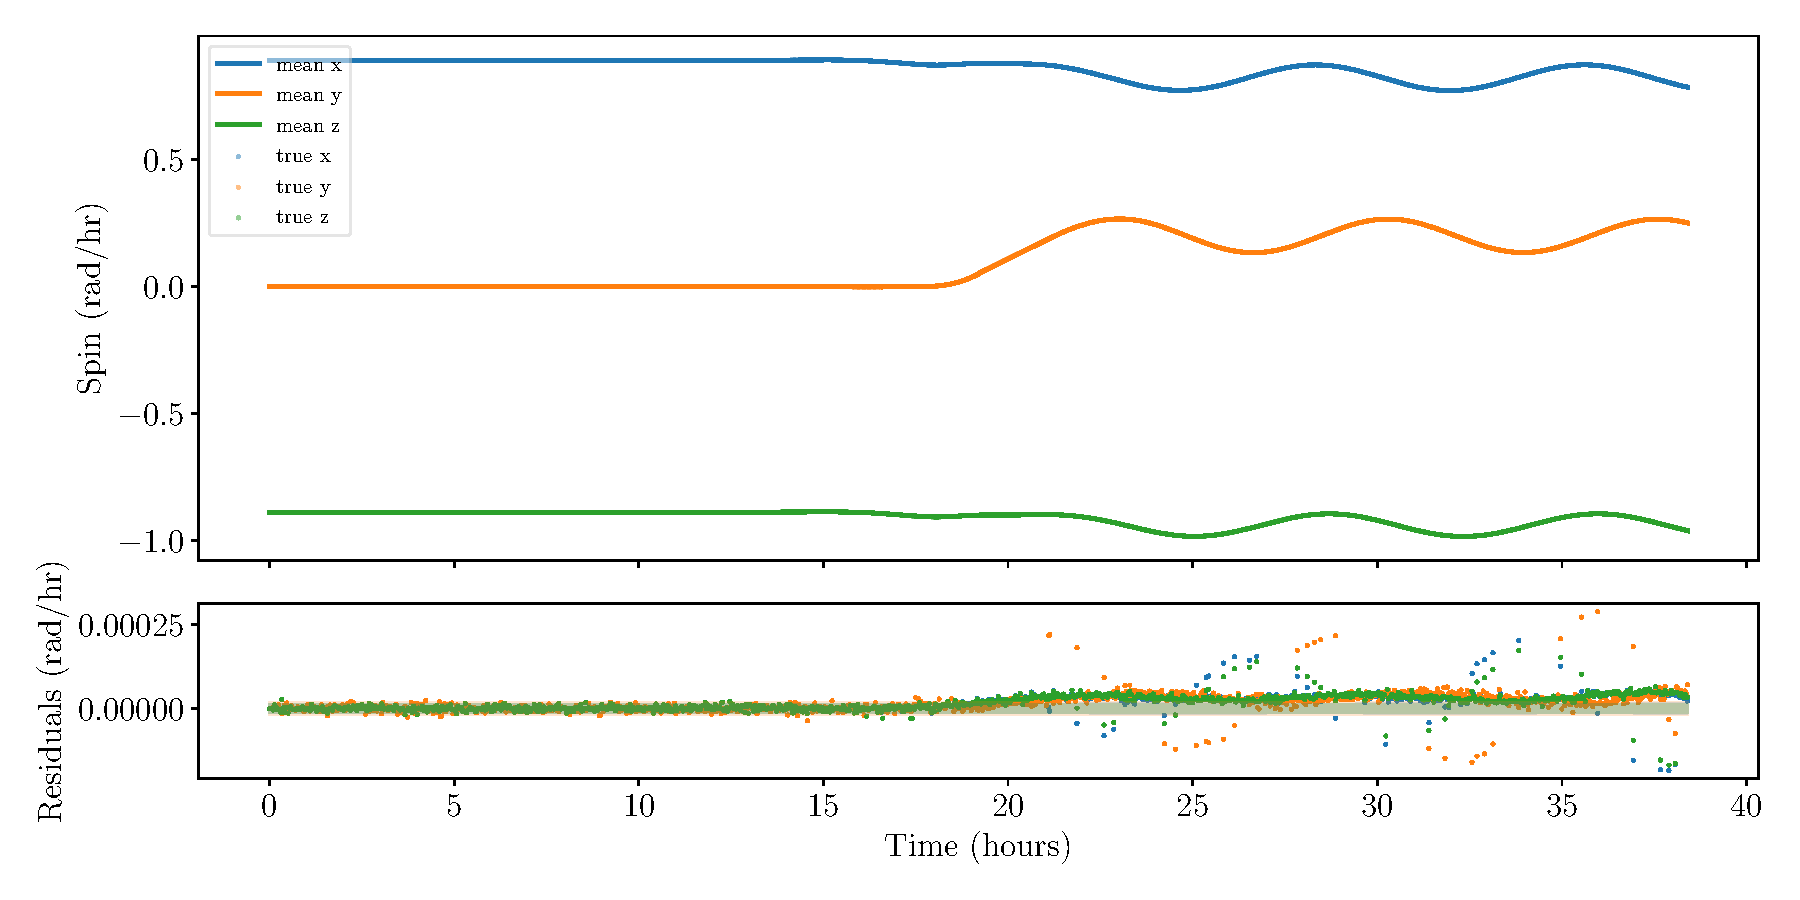
\includegraphics[width=0.7\textwidth]{example-residuals.pdf}
  \caption{Data, best fit results, and residuals for a fit to synthetic data simulated for an asymmetric reference asteroid with $\sigma_\theta = 10^{-5}$. The standard deviation of the data is plotted as an uncertainty band in the residuals plot, but these do not capture covariance between data points, so that the fact that many residuals lie outside the band does not disqualify the fit, which has a reduced $\chi^2$ value of 0.68.}
  \label{fig:example-residuals}
\end{figure}

Figure \ref{fig:example-corner} shows a corner plot of the ten fitted parameters' posterior distributions, both marginalized to be a function of one variable and of two. The true parameters are shown as lines.

\begin{figure}
  \centering
  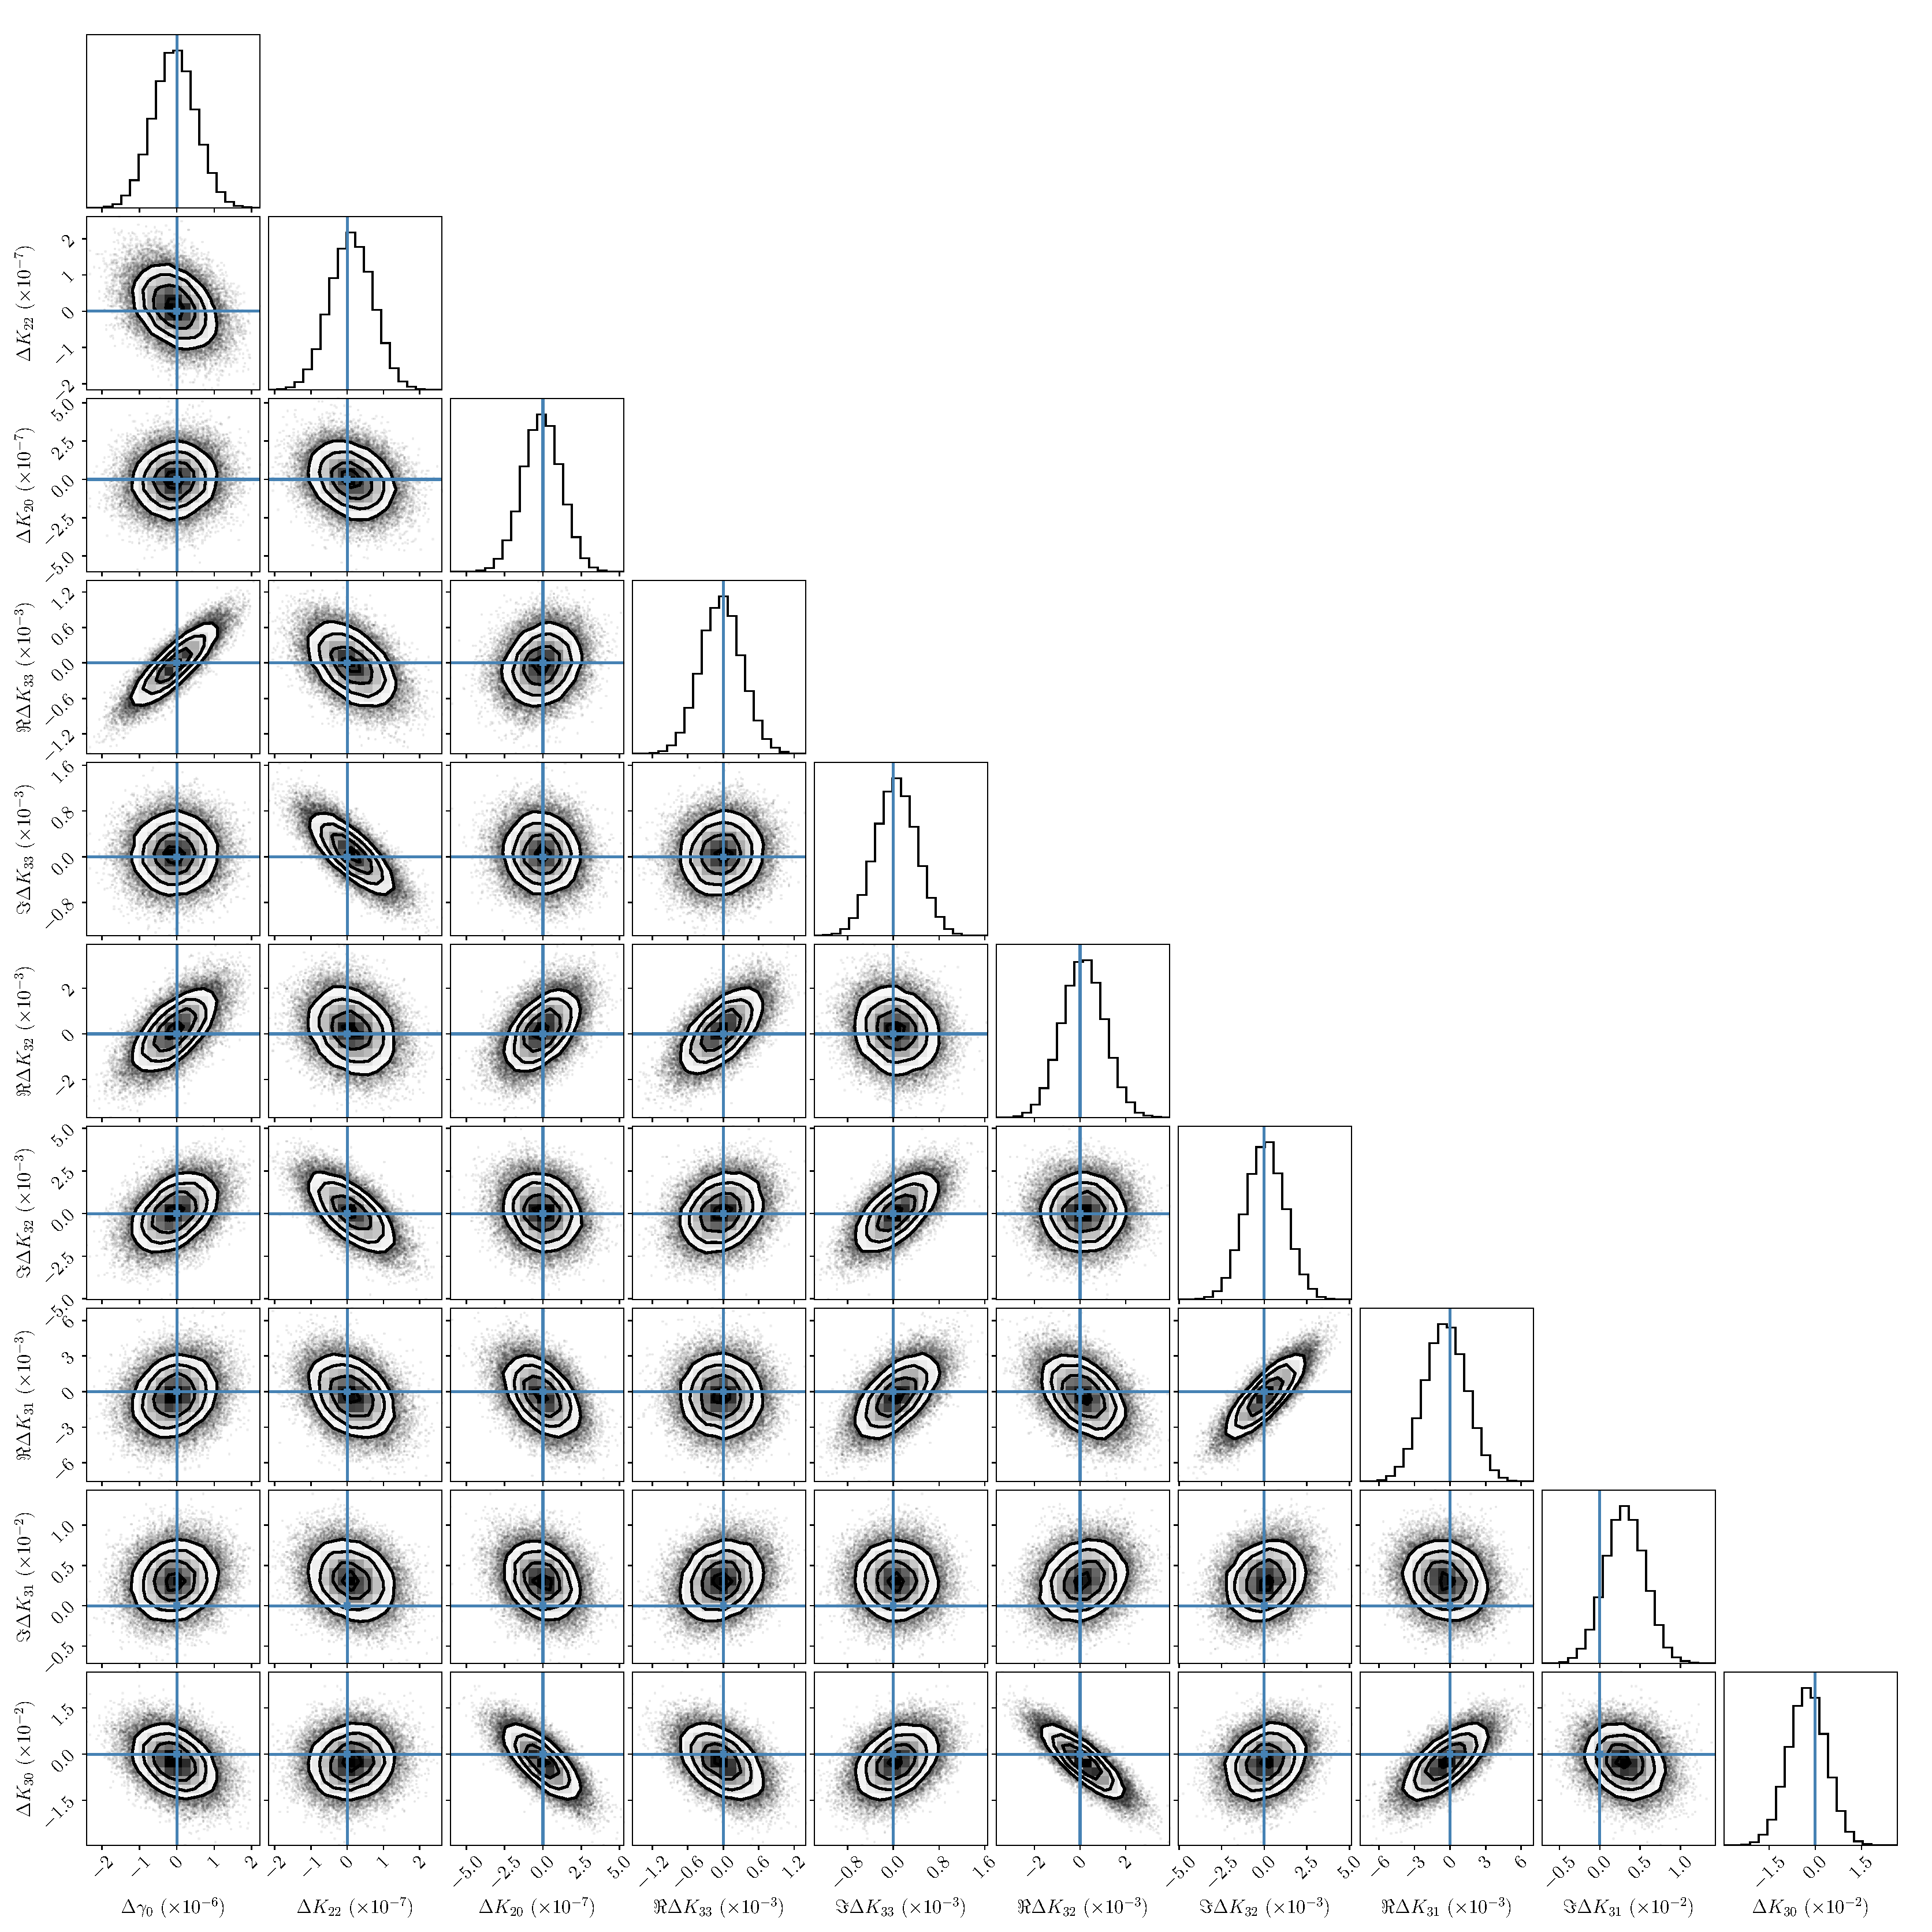
\includegraphics[width=\textwidth]{example-corner.pdf}
  \caption{A corner plot for the fit results ten parameters to synthetic data simulated for an asymmetric reference asteroid with $\sigma_\theta = 10^{-5}$. Marginal posterior PDFs for each parameter are shown (histograms) along with two-dimensional PDFs (contours). Individual points in the contours are samples from the MCMC fit, and the contours enclose 1-, 2-, and 3-$\sigma$ of them. True values (which are zero here due to the parameters being displayed relative to the true values) are also shown (blue lines).}
  \label{fig:example-corner}
\end{figure}

Figure \ref{fig:example-residuals} demonstrates that a good fit to data was achieved, despite the small error bars and strong dependence of the model on initial conditions. Figure \ref{fig:example-corner} shows that the posterior distributions are largely Gaussian-distributed, with several of the parameters strongly correlated. The true values lie within $2\sigma$ contours in most cases, as expected. Parameters are computed to very high accuracy --- $O(10^{-7})$ for $\gamma_0$ and $O(10^{-9})$ for $K_{2m}$ (the first tier of parameters as ordered by the sensitivity of the asteroid system to their values), and $O(10^{-4})-O(10^{-6})$ for $K_{3m}$. These ranges should be compared to the width of the prior distributions for these parameters, which is $O(1)$ for all. The success of this fit demonstrates that these higher order parameters can be fitted to data as long as good enough precision on the data is achieved.



\section{Gaussianity of Parameter Posterior Distributions}
\label{app:gaussian-posteriors}



\bibliography{asteroids}{}
\bibliographystyle{aasjournal}



\end{document}
